\documentclass[preprint,12pt]{elsarticle}
\usepackage{amsmath,amssymb,amsthm,amsfonts}
\usepackage{stix}
\usepackage{booktabs,graphicx,xcolor,float}
\usepackage[colorlinks=true,linkcolor=blue,citecolor=blue]{hyperref}
\newtheorem{theorem}{Theorem}
\newtheorem{proposition}[theorem]{Proposition}
\newtheorem{corollary}[theorem]{Corollary}
\theoremstyle{remark}
\newtheorem{remark}{Remark}
\newfloat{algorithm}{tbp}{loa}
\floatname{algorithm}{Algorithm}
\newcommand{\todo}[1]{\textcolor{red}{\textbf{[TODO: #1]}}}
\newcommand{\proofin}[1]{\hfill{\small\emph{(Proof: Appendix~\ref{#1}.)}}}
\journal{Computer Methods in Applied Mechanics and Engineering}

\begin{document}
\begin{frontmatter}
\title{Integrated-Haar wavelet collocation revisited: fast tensor solvers, fourth-order
energy-stable phase-field schemes with sharp interfaces, and automatic refinement for elastic corner singularities}

\author[inst1]{Farshid Mossaiby\corref{cor1}}
\ead{mossaiby@eng.ui.ac.ir}
\cortext[cor1]{Corresponding author}
\affiliation[inst1]{organization={Department of Civil Engineering, University of Isfahan},
            city={Isfahan}, postcode={81744-73441}, country={Iran}}

\begin{abstract}
The Haar wavelet collocation method (HWCM) is popular in engineering because it is simple: the
highest derivative of the unknown is expanded in Haar functions and integrated. In two dimensions,
however, it is usually solved through a dense matrix of size $N^2\times N^2$, it is second-order
accurate, and graded grids must be tuned by hand. We show that none of these limitations is
intrinsic. An exact three-term relation between the nodal values and the Haar coefficients turns
the dense HWCM matrices into tridiagonal ones. Two- and three-dimensional problems then reduce to
tensor (Sylvester) equations that are solved by fast diagonalization or, on uniform grids, by fast
cosine transforms. A one-line correction raises the accuracy to fourth order at no extra cost.
Building on this structure, we construct Allen--Cahn and Cahn--Hilliard solvers that conserve mass
exactly and are provably energy-stable for any time step. Each time step costs two fast transforms.
With a stabilization term, they resolve interfaces as thin as about two nodes per
$\sqrt2\varepsilon$ on $1024^2$ grids. For plane elastostatics with Dirichlet and traction
boundaries, a preconditioned Krylov solver converges in a number of iterations independent of the
mesh, and automatic anisotropic refinement driven by Haar detail coefficients recovers the optimal
convergence rate at Mode-I corner singularities. On identical grids it reaches the accuracy of
biquadratic finite elements with about one quarter of the unknowns, and with solve times one to two
orders of magnitude shorter than a sparse direct solver. We also compare against finite-difference,
compact and pseudo-spectral discretizations, and state where each is preferable. All proofs are
collected in appendices; the main text
states each result together with its practical meaning. The accompanying open-source code runs
unchanged on CPUs (NumPy) and is designed for GPUs (CuPy).
\end{abstract}

\begin{keyword}
Haar wavelet collocation \sep fast diagonalization \sep Allen--Cahn \sep Cahn--Hilliard \sep
sharp interfaces \sep energy stability \sep corner singularities \sep adaptive refinement \sep GPU
\end{keyword}
\end{frontmatter}

%==========================================================================
\section{Introduction}
%==========================================================================
Since the work of Chen and Hsiao~\cite{chen1997haar} and the systematic developments of
Lepik~\cite{lepik2005numerical,lepik2007application,lepik2011solving,lepik2014book}, the Haar wavelet
collocation method (HWCM) has become a popular tool in applied mechanics, in particular for beams,
plates, shells and functionally graded structures~\cite{majak2015accuracy,majak2015convergence,majak2018higher}.
The highest derivative of the unknown is expanded in Haar functions, lower derivatives follow by exact
integration, boundary conditions fix the integration constants, and the equation is collocated at cell
midpoints. Majak et al.\ proved second-order convergence~\cite{majak2015convergence} and proposed a
higher-order variant (HOHWM)~\cite{majak2018higher}, which has been applied to nonlinear ordinary
differential equations~\cite{ratas2021solving}. Non-uniform Haar
wavelets~\cite{dubeau2004nonuniform,lepik2008nonuniform} have been used on graded grids, including
two-dimensional problems with boundary layers~\cite{oruc2019nonuniform}.

Three limitations recur in this literature:
\begin{enumerate}
\item In two dimensions all collocation equations are assembled into one dense $N^2\times N^2$
matrix~\cite{lepik2011solving,oruc2019nonuniform}, whose solution costs $O(N^6)$ operations. This is
infeasible beyond about $64\times64$ cells (Table~\ref{tab:cost}).
\item Graded grids must be chosen \emph{a priori}, for example through a grading parameter re-tuned for
every value of a small parameter~\cite{oruc2019nonuniform}.
\item There is no stability theory for nonlinear time-dependent problems. In particular, no HWCM for
phase-field models with guaranteed energy decay and mass conservation is available.
\end{enumerate}

The key observation of this paper is that the integrated-Haar trial space consists of smooth ($C^1$)
piecewise-quadratic functions. HWCM is therefore a quadratic-spline collocation
method~\cite{houstis1988quadratic,christara1994quadratic,christara2006optimal,christara2002fast}, and
it uses the same function space as quadratic isogeometric
collocation~\cite{auricchio2010isogeometric,schillinger2013isogeometric,anitescu2015isogeometric,gomez2016variational}.
Exploiting this connection, we make the following contributions.
\begin{enumerate}
\item \textbf{A three-term identity} (Theorem~\ref{thm:identity}) replaces the dense operational
matrices of HWCM by tridiagonal matrices on arbitrary grids. For uniform partitions the relation is
classical in quadratic-spline collocation~\cite{houstis1988quadratic}, and non-uniform partitions are
analysed in~\cite{christara2006optimal}. Here it is written in HWCM variables, with Dirichlet and Neumann end rows, and used as the basis of
everything that follows. As a by-product, unique solvability holds on \emph{every} grid, by a short
diagonal-dominance argument; existence and uniqueness for optimal QSC on non-uniform partitions were
previously established under some conditions on the partition~\cite{christara2006optimal}.
\item \textbf{Fast solvers}: Sylvester equations solved by fast diagonalization~\cite{lynch1964direct},
or by discrete cosine/sine transforms on uniform grids. Every time step of a phase-field computation
reduces to dense matrix products or fast transforms, which map directly onto GPUs.
\item \textbf{A fourth-order correction} (Theorem~\ref{thm:fourth}). It is the PDE counterpart of
HOHWM, but it requires no extra integration constants and preserves the fast solvers.
\item \textbf{Phase-field solvers with guarantees}: exact discrete mass conservation and an
unconditional energy law for a stabilized SAV-BDF2 scheme (Theorem~\ref{thm:energy}). Examples with
very thin interfaces quantify how many nodes an interface needs.
\item \textbf{Elastostatics with Dirichlet and traction edges}: mesh-independent preconditioned GMRES,
and automatic anisotropic refinement driven by Haar detail coefficients that recovers the optimal rate
at corner singularities. One-dimensional adaptive QSC with mapping functions was developed
in~\cite{christara2006adaptive}; here refinement is two-dimensional, anisotropic and driven directly by
the Haar coefficients.
\item \textbf{Honest comparisons}: with biquadratic ($Q_2$) finite elements on identical grids, and with
3-point, compact (Pad\'e) and pseudo-spectral discretizations of the phase-field models.
\end{enumerate}

\paragraph{How to read this paper} Section~\ref{sec:method} explains the method in one dimension, and
Section~\ref{sec:tensor} explains how it extends to 2D/3D with fast solvers. Sections~\ref{sec:pf}
and~\ref{sec:elast} present the phase-field and elasticity solvers, each with an algorithm box.
Section~\ref{sec:results} reports the numerical results, and Section~\ref{sec:guide} collects
practical guidelines. Every theorem is stated in the main text together with its practical meaning;
the proofs are in Appendices~\ref{app:ops} and~\ref{app:energy}. The scope is limited to rectangular
(tensor-product) domains, where the fast solvers apply; Section~\ref{sec:limits} discusses
extensions.

%==========================================================================
\section{The method in one dimension}\label{sec:method}
%==========================================================================
\subsection{From Haar coefficients to nodal values}
Let $a=t_0<t_1<\dots<t_N=b$ be the grid, with cells $I_k=[t_{k-1},t_k]$ of width $h_k$, midpoints
$m_k$, and midpoint spacings $d_k=(h_k+h_{k+1})/2$. Classical HWCM writes
$u''(x)=\sum_ia_i\,\mathsf h_i(x)$ with (possibly non-uniform~\cite{dubeau2004nonuniform}) Haar
functions $\mathsf h_i$ and integrates twice. On a given grid, the Haar functions span exactly the
piecewise constants, so the Haar coefficients $a_i$ carry the same information as the cell values
$c_k=u''|_{I_k}$; the two are related by the (orthogonal, on uniform dyadic grids) Haar transform.
The double integral of a piecewise constant is a piecewise quadratic with continuous slope.
Hence the HWCM trial space is
\[
\mathcal S_h=\{s\in C^1[a,b]:\ s|_{I_k}\ \text{is quadratic}\},
\]
the space of $C^1$ quadratic splines on the grid. We work with the HWCM collocation values
$U_k=s(m_k)$ as unknowns. Haar coefficients are only needed for the refinement indicator
(Section~\ref{sec:adapt}).

\subsection{The three-term identity}
\begin{theorem}[Three-term identity]\label{thm:identity}
For every $s\in\mathcal S_h$, with $U_k=s(m_k)$ and $c_k=s''|_{I_k}$, and for $2\le k\le N-1$,
\begin{equation}\label{eq:interior}
\frac{U_{k+1}-U_k}{d_k}-\frac{U_k-U_{k-1}}{d_{k-1}}
=\frac{h_{k-1}^2}{8d_{k-1}}c_{k-1}+\Big(h_k-\frac{h_k^2}{8d_{k-1}}-\frac{h_k^2}{8d_k}\Big)c_k+\frac{h_{k+1}^2}{8d_k}c_{k+1}.
\end{equation}
At the left end, with $g_0=s(a)$,
\begin{align}
\frac{U_2-U_1}{d_1}-\frac{2(U_1-g_0)}{h_1}&=\Big(\frac{3h_1}{4}-\frac{h_1^2}{8d_1}\Big)c_1+\frac{h_2^2}{8d_1}c_2 &&\text{(value $g_0$ prescribed)},\label{eq:dirrow}\\
\frac{U_2-U_1}{d_1}&=\Big(h_1-\frac{h_1^2}{8d_1}\Big)c_1+\frac{h_2^2}{8d_1}c_2 &&\text{(if } s'(a)=0),\label{eq:neurow}
\end{align}
and symmetrically at the right end. In matrix form, $LU+b_0g_0+b_1g_1=Ac$ with tridiagonal matrices
$L$ (a three-point difference) and $A$ (a three-point average).
\proofin{app:identity}
\end{theorem}

\paragraph{What this means in practice}
\begin{itemize}
\item The second derivative at the collocation points is $c=D_2U+e_0g_0+e_1g_1$, with
$D_2=A^{-1}L$ and $e_i=A^{-1}b_i$. Only two tridiagonal matrices need to be assembled, instead of the
dense integration matrices of HWCM. $A$ is invertible on every grid, and the 1D Dirichlet collocation
problem always has a unique solution (Corollary~\ref{cor:ops}).
\item The slope at the collocation points is available in closed form:
$s'(m_k)=\sigma_0+\sum_{j<k}c_jh_j+\tfrac12c_kh_k$, with end slope
$\sigma_0=2(U_1-g_0)/h_1-c_1h_1/4$. This defines the first-derivative matrix $D_1$, and also the
end slopes needed for traction conditions (Section~\ref{sec:traction}).
\item We verified $D_2$ and $D_1$ against the classical integrated-Haar matrices on random
non-uniform grids; they agree to round-off (\texttt{tests/test\_core.py}).
\end{itemize}

\begin{corollary}\label{cor:ops}
On every grid, $A$ has a positive diagonal and is strictly diagonally dominant by columns, hence
invertible. With values prescribed at both ends, the collocation problem $s''(m_k)=f(m_k)$ has a
unique solution.
\proofin{app:identity}
\end{corollary}

\begin{algorithm}[t]\small\hrule\smallskip
\textbf{Algorithm 1: one-dimensional operators} (\texttt{ihaar/core.py, Grid1D})\\[2pt]
\textbf{Input:} knots $t_0<\dots<t_N$; end types (value prescribed or zero slope).
\begin{enumerate}
\item Compute $h_k$, $m_k$, $d_k$. Assemble the tridiagonal $L$ and $A$ from~\eqref{eq:interior}--\eqref{eq:neurow}.
\item Factorize $A$ (tridiagonal LU). Set $D_2=A^{-1}L$ and the boundary vectors $e_i=A^{-1}b_i$.
\item First derivative: $D_1=\mathbf 1 r^{\mathsf T}+T D_2$, where $T_{kj}=h_j$ $(j<k)$ and $T_{kk}=h_k/2$, and $r$ encodes $\sigma_0$.
\item End slopes $s'(a)=\sigma_0$ and $s'(b)=\sigma_0+\sum_kh_kc_k$ as row vectors (for traction conditions).
\end{enumerate}
\hrule
\end{algorithm}

\subsection{Uniform grids: symmetry, cosine transforms, and a fourth-order correction}
\begin{proposition}\label{prop:uniform}
On a uniform grid ($h_k\equiv h$), $D_2$ is a symmetric matrix,
\begin{equation}\label{eq:D2}
D_2=\frac{8}{h^2}\,\delta^2\,(8I+\delta^2)^{-1},
\end{equation}
where $\delta^2$ is the usual three-point second-difference matrix (first/last diagonal entry $-3$ for
prescribed values, $-1$ for zero slope). Its eigenvectors are the DST-II (prescribed values) or
DCT-II (zero slope) vectors, and its eigenvalues
$\lambda_k=8\mu_k/(h^2(8+\mu_k))$, with $\mu_k=-4\sin^2(\pi k/2N)$, lie in $[-8/h^2,0]$.
\proofin{app:uniform}
\end{proposition}

\paragraph{What this means in practice} On uniform grids, HWCM behaves like a well-structured finite
difference scheme. Systems can be solved with fast cosine/sine transforms ($O(N\log N)$ per line).
The discrete Laplacian is symmetric and negative, which is what the energy-stability results of
Section~\ref{sec:pf} rest on. Its largest eigenvalue magnitude, $8/h^2$, is twice that of the
standard 3-point difference.

\begin{theorem}[Fourth-order correction]\label{thm:fourth}
On a uniform grid, for smooth $u$ satisfying zero-slope (Neumann) conditions with all odd normal
derivatives vanishing, or periodic conditions,
\begin{equation}\label{eq:D24}
D_2U=u''(m)-\tfrac{h^2}{24}u^{(4)}(m)+O(h^4),\qquad
D_2^{(4)}U=u''(m)+O(h^4),\quad\text{with}\quad D_2^{(4)}:=D_2+\tfrac{h^2}{24}D_2^2 .
\end{equation}
$D_2^{(4)}$ has the same eigenvectors as $D_2$ and eigenvalues
$\lambda_k+h^2\lambda_k^2/24\in[-\tfrac{16}{3h^2},0]$, so it is also symmetric and negative.
The same holds for prescribed values when the even derivatives vanish at the ends.
\proofin{app:fourth}
\end{theorem}

\paragraph{What this means in practice}
\begin{itemize}
\item The error constant of $D_2$, $-h^2/24$, is half that of the 3-point difference ($+h^2/12$), so
plain HWCM is about twice as accurate as finite differences on the same grid (Fig.~\ref{fig:res}).
\item The correction~\eqref{eq:D24} costs nothing extra: in the transform domain it only changes the
eigenvalues.
\item The condition on the boundary data holds for the Allen--Cahn and Cahn--Hilliard equations with
zero-flux conditions. For general prescribed values, the end rows keep an $O(h^2)$ error and the
overall order stays two (Table~\ref{tab:poisson}).
\end{itemize}

\begin{remark}[Relation to the classical compact scheme]
The rational variant $D_2(I-\tfrac{h^2}{24}D_2)^{-1}$ reduces exactly to the classical fourth-order
compact (Pad\'e) operator $\delta^2(I+\delta^2/12)^{-1}/h^2$, as follows directly from~\eqref{eq:D2}.
The polynomial form~\eqref{eq:D24} has a slightly larger leading error constant, $0.0059\,\theta^6$
against $\theta^6/240$ in symbol terms, so it is about $1.4\times$ less accurate
(Table~\ref{tab:compare}). In exchange, it needs no inverse, which matters on non-uniform grids and
whenever the operator is applied rather than inverted.
\end{remark}

\begin{proposition}[Exact mass conservation]\label{prop:mass}
With zero-slope ends, on any grid, $h^{\mathsf T}D_2=0$ with $h=(h_k)$. On uniform grids,
moreover, $h\sum_kU_k$ equals the exact integral of the spline.
\proofin{app:mass}
\end{proposition}

%==========================================================================
\section{Two and three dimensions: fast tensor solvers}\label{sec:tensor}
%==========================================================================
On a rectangle, the trial space is the tensor product of the 1D spaces in $x$ and $y$, and the unknowns
form a matrix $U_{ij}=u_h(m^x_i,m^y_j)$. Along every grid line, $u_h$ is a 1D spline, so the 1D
operators apply line by line:
\begin{equation}\label{eq:tensorops}
U_{xx}=D_2^xU+e_0^x g_L^{\mathsf T}+e_1^x g_R^{\mathsf T},\qquad
U_{yy}=U(D_2^y)^{\mathsf T}+g_B(e_0^y)^{\mathsf T}+g_T(e_1^y)^{\mathsf T},
\end{equation}
where $g_L,g_R,g_B,g_T$ are the boundary values at the edge midpoints. Mixed derivatives are
computed as $U_{xy}=\partial_y(U_x)$, using the corner values for the slopes along the edges. All
derivatives are then exact derivatives of a single biquadratic $C^1$ spline. Classical
two-dimensional HWCM, which expands $u_{xxyy}$~\cite{lepik2011solving,oruc2019nonuniform}, uses
essentially the same trial space, but solves it through a dense $N^2\times N^2$ system.

\paragraph{Sylvester equations and fast diagonalization}
For $\alpha u_{xx}+\beta u_{yy}+\gamma u=f$, collocation gives the Sylvester equation
$\alpha D_2^xU+\beta U(D_2^y)^{\mathsf T}+\gamma U=\tilde F$. With $D_2^x=V_x\Lambda_xV_x^{-1}$ and
$D_2^y=V_y\Lambda_yV_y^{-1}$,
\begin{equation}\label{eq:fdm}
U=V_x\Big[\big(V_x^{-1}\tilde FV_y^{-\mathsf T}\big)\oslash\big(\alpha\lambda^x_i+\beta\lambda^y_j+\gamma\big)_{ij}\Big]V_y^{\mathsf T},
\end{equation}
where $\oslash$ is entrywise division. This is four matrix products after a one-time
eigendecomposition~\cite{lynch1964direct}. In 3D, mode products give $O(N^4)$. On uniform grids, the
transforms are DCT/DST (Proposition~\ref{prop:uniform}), and the cost is $O(N^d\log N)$. On graded
grids, $D_2=A^{-1}L$ is not symmetric; we check that its spectrum is real and monitor the
conditioning $\kappa(V)$ of the eigenvector matrix (below 25 in all computations here). If the check
fails, the Bartels--Stewart algorithm~\cite{bartels1972solution} is available as a fallback. Fast
Sylvester solvers of this kind are also used in isogeometric preconditioning~\cite{sangalli2016isogeometric}.

\paragraph{GPU implementation}
All 1D factorizations are computed once, on the host, and moved to the device. Every subsequent
operation is a dense matrix product (GEMM), a batched fast cosine transform, or a pointwise operation.
No sparse data structure is needed. The code takes the array module (\texttt{numpy} or \texttt{cupy})
as a parameter, so the same code path runs on CPU and GPU.

%==========================================================================
\section{Phase-field solvers}\label{sec:pf}
%==========================================================================
We consider the Allen--Cahn (AC) and Cahn--Hilliard (CH) equations on $\Omega=(0,1)^d$ with zero-flux
conditions,
\begin{equation}
u_t=-\mathcal G\mu,\qquad \mu=-\varepsilon^2\Delta u+f(u),\qquad f(u)=u^3-u,\qquad
\mathcal G=I\ \text{(AC)},\ \ \mathcal G=-\Delta\ \text{(CH)},
\end{equation}
which are gradient flows of the free energy
$E(u)=\int_\Omega\tfrac14(u^2-1)^2+\tfrac{\varepsilon^2}{2}|\nabla u|^2$. The parameter $\varepsilon$ sets the
interface thickness; across an equilibrium interface, $u\approx\tanh(d/\sqrt2\varepsilon)$, where $d$ is the
signed distance. On a uniform grid, $\Delta_h$ is the tensor sum of $D=D_2$ or $D=D_2^{(4)}$,
$K=-\Delta_h$, $\langle v,w\rangle_h=h^d\sum vw$, and the discrete energy is
$E_h(u)=\langle F(u),1\rangle_h+\tfrac{\varepsilon^2}{2}\langle Ku,u\rangle_h$.

\paragraph{Stabilized SAV-BDF2 scheme}
Following the scalar auxiliary variable (SAV) approach~\cite{shen2018scalar}, let
$r\approx\sqrt{E_{1,h}+C}$ with $E_{1,h}=\langle F(u),1\rangle_h$ and $C>0$. Let $\bar u=2u^n-u^{n-1}$,
$\bar b=f(\bar u)/\sqrt{E_{1,h}(\bar u)+C}$, and let $S\ge0$ be a stabilization constant. Then
\begin{align}
\frac{3u^{n+1}-4u^n+u^{n-1}}{2\Delta t}&=-G_h\mu^{n+1},\qquad
\mu^{n+1}=\varepsilon^2Ku^{n+1}+S(u^{n+1}-\bar u)+r^{n+1}\bar b,\label{eq:sav1}\\
3r^{n+1}-4r^n+r^{n-1}&=\tfrac12\langle\bar b,3u^{n+1}-4u^n+u^{n-1}\rangle_h,\label{eq:sav2}
\end{align}
with $G_h=I$ (AC) or $K$ (CH). The first step uses BDF1. Algorithm~2 shows that a step consists of one
forward and one inverse transform, plus the scalar update of $r$.

\begin{theorem}[Solvability, mass, energy]\label{thm:energy}
For every $\Delta t>0$ and $S\ge0$, the scheme has a unique solution. For CH, the discrete mass
$\langle u^n,1\rangle_h$, which equals the exact integral of the spline, is constant. The modified energy
\[
\tilde E^{n+1}=\tfrac{\varepsilon^2}{4}\big(\|u^{n+1}\|_K^2+\|2u^{n+1}-u^n\|_K^2\big)
+\tfrac12\big((r^{n+1})^2+(2r^{n+1}-r^n)^2\big)+\tfrac S2\|u^{n+1}-u^n\|_h^2
\]
never increases: $\tilde E^{n+1}\le\tilde E^n$. This holds for both $D_2$ and $D_2^{(4)}$.
\proofin{app:energy}
\end{theorem}

\paragraph{What this means in practice, and why $S$ matters}
Theorem~\ref{thm:energy} guarantees that the computation cannot blow up in the modified energy, for any
time step. For thin interfaces, however, this guarantee alone is weak. It bounds
$\|\nabla u\|^2$ only by roughly $\tilde E/\varepsilon^2$, which allows large values of $u$ when
$\varepsilon$ is small. Table~\ref{tab:savstab} shows this happening for $\varepsilon=0.0015$: plain SAV
($S=0$) produces $|u|\approx 30$--$70$ within 150 steps, even though $\tilde E$ decreases at every step
exactly as proved. With $S=4$ the same time steps give $|u|\le1.04$, decreasing energy, and an SAV
ratio $\xi=r/\sqrt{E_{1,h}+C}$ equal to 1 to five digits. We therefore recommend $S\approx4$ and
monitoring $\xi$, as a deviation from 1 is an inexpensive warning sign~\cite{shen2018scalar}.

\begin{algorithm}[t]\small\hrule\smallskip
\textbf{Algorithm 2: one SAV-BDF2 time step} (\texttt{ihaar/phasefield.py})\\[2pt]
\textbf{Precomputed:} transform (DCT-II, or eigenvectors $V$); symbols $\hat\lambda$ of $-K$;
$\hat G=1$ (AC) or $\hat\lambda$ (CH); $\hat S_2=3+2\Delta t\,\hat G(\varepsilon^2\hat\lambda+S)$.\\
\textbf{Stored:} $\hat u^n,\hat u^{n-1}$, $u^n,u^{n-1}$, $r^n,r^{n-1}$.
\begin{enumerate}
\item $\bar u=2u^n-u^{n-1}$; \ $\bar b=f(\bar u)/\sqrt{E_{1,h}(\bar u)+C}$; \ $\hat{\bar b}=\mathcal T\bar b$ \hfill (one forward transform)
\item $\hat g=4\hat u^n-\hat u^{n-1}$; \ $\hat p=(\hat g+2\Delta t\,S\hat G\,\hat{\bar u})/\hat S_2$; \ $\hat q=-2\Delta t\,\hat G\hat{\bar b}/\hat S_2$
\item $r^{n+1}=\dfrac{4r^n-r^{n-1}+\tfrac12\langle\hat{\bar b},3\hat p-\hat g\rangle}{3-\tfrac32\langle\hat{\bar b},\hat q\rangle}$ \hfill (inner products in the orthonormal transform domain)
\item $\hat u^{n+1}=\hat p+r^{n+1}\hat q$; \ $u^{n+1}=\mathcal T^{-1}\hat u^{n+1}$ \hfill (one inverse transform)
\end{enumerate}
\hrule
\end{algorithm}

%==========================================================================
\section{Elastostatics: boundary conditions, solver and adaptivity}\label{sec:elast}
%==========================================================================
\subsection{Collocation and preconditioned GMRES}
For plane strain with Lam\'e constants $\lambda_L,\mu$ and body force $\mathbf b$, we collocate the
Navier equations
\begin{equation}
(\lambda_L+2\mu)u_{xx}+\mu u_{yy}+(\lambda_L+\mu)v_{xy}+b_x=0,\qquad
\mu v_{xx}+(\lambda_L+2\mu)v_{yy}+(\lambda_L+\mu)u_{xy}+b_y=0
\end{equation}
at the interior midpoints, using the operators of Section~\ref{sec:tensor}. The coupling terms
prevent a single Sylvester solve. We therefore use right-preconditioned GMRES, with the decoupled
operator
$\mathrm{diag}\big((\lambda_L+2\mu)D_2^x\oplus\mu D_2^y,\ \mu D_2^x\oplus(\lambda_L+2\mu)D_2^y\big)$
as preconditioner. Here $A\oplus B$ denotes $A\otimes I+I\otimes B$, and each preconditioner
application is two fast-diagonalization solves~\eqref{eq:fdm}.

\subsection{Traction boundary conditions}\label{sec:traction}
On a traction edge, the edge-midpoint displacements are unknowns, and
$\boldsymbol\sigma(\mathbf u_h)\mathbf n=\mathbf t$ is collocated at the edge midpoints:
\begin{itemize}
\item The normal derivative at the edge is the end slope of Algorithm~1 (step~4), applied along the
grid lines ending on the edge.
\item The tangential derivative is $D_1$ applied to the edge values.
\item A corner shared with a Dirichlet edge takes the Dirichlet value. A corner shared by two traction
edges has two unknowns, closed by the two normal-stress conditions $\sigma_{xx}=t_x$ and
$\sigma_{yy}=t_y$.
\end{itemize}
In the preconditioner, the traction rows are replaced by zero-slope rows~\eqref{eq:neurow}. Eliminating
the edge value gives exactly the Neumann version of Theorem~\ref{thm:identity}, so the fast solver
applies unchanged; the $u$--$v$ coupling in the traction rows is left to GMRES.

\begin{remark}[No ``enhanced'' collocation needed]
For quadratic isogeometric collocation at Greville points, pointwise traction conditions degrade
accuracy, and an ``enhanced'' boundary equation, which adds $\alpha h$ times the PDE residual, is
recommended~\cite{delorenzis2015isogeometric}. For midpoint collocation we observe no loss of order.
In 1D, every $\alpha$ gives second order; the standard $\alpha=1/4,1/2$ increase the error, and
$\alpha=-1/12$ reduces it by a factor of three (Table~\ref{tab:enh1d}). In 2D, plain collocation
($\alpha=0$) is second order for all tested configurations (Table~\ref{tab:tracsmooth}).
\end{remark}

\subsection{Automatic refinement from Haar detail coefficients}\label{sec:adapt}
On a uniform dyadic grid, the finest-level Haar coefficient of $u''$ is proportional to the jump of
$u''$ between two sibling cells. For a $C^1$ quadratic, such a jump is about $h\,u'''$, so it measures
the local error of the gradient. We use jumps across all interior knots, which is well defined on graded
grids, and define for each $x$-cell
\begin{equation}\label{eq:indicator}
\eta^x_i{}^2=h^x_i{}^3\sum_jh^y_j\,\tfrac12\Big([\![u_{xx}]\!]_{i-\frac12,j}^2+[\![u_{xx}]\!]_{i+\frac12,j}^2\Big),
\end{equation}
summed over both displacement components, and analogously $\eta^y_j$. The indicator is heuristic: we
do not prove reliability or efficiency bounds, but it tracks the true error closely in all tests.
Algorithm~3 summarizes the loop.

\begin{algorithm}[t]\small\hrule\smallskip
\textbf{Algorithm 3: adaptive elastostatics} (\texttt{ihaar/elasticity\_bc.py})
\begin{enumerate}
\item Start from a uniform tensor grid, e.g.\ $8\times8$ cells.
\item Build the 1D operators (Algorithm~1) and the preconditioner factorizations; solve with
right-preconditioned GMRES (tolerance $10^{-10}$, restart 60--80).
\item Compute $\eta^x_i$ and $\eta^y_j$ from~\eqref{eq:indicator}.
\item Mark the smallest set of 1D cells (both directions together) carrying a fraction $\theta=0.6$ of
$\sum\eta^2$ (D\"orfler marking~\cite{dorfler1996convergent}); bisect them.
\item Bisect further until neighbouring cells differ in size by at most a factor of 2; return to step 2.
\end{enumerate}
\hrule
\end{algorithm}

%==========================================================================
\section{Numerical results}\label{sec:results}
%==========================================================================
All computations were run on one core of a virtual x86 CPU with NumPy~2.4 and SciPy~1.17 in double
precision. Every table and figure is produced by \texttt{experiments/run\_all.py}, and all tables are
typeset automatically from the stored results by \texttt{experiments/make\_tables.py}.

\subsection{Verification and cost of a linear solve}
Table~\ref{tab:poisson} reports the maximum nodal errors for $-\Delta u=f$ with prescribed values,
$u=e^x\sin\pi y+x^2y$, on uniform and Chebyshev-graded grids, and for $(I-\Delta)u=f$ with zero-slope
conditions, $u=\cos\pi x\cos2\pi y+0.3\cos3\pi x$. The plain operator is second order on both grid types.
The corrected operator is fourth order when its conditions hold, reaching $3\times10^{-10}$ at $N=512$.
Table~\ref{tab:cost} compares the wall time of one solve. Classical dense HWCM needs 1.2~s at $N=64$
and is infeasible beyond that, whereas the cosine-transform solver handles $10^6$ unknowns in 0.03~s.
The fast-diagonalization times exclude the one-time $O(N^3)$ eigendecomposition, which is amortized
over many solves.

\begin{table}[t]\centering\footnotesize
\caption{Maximum nodal error and observed rates.}\label{tab:poisson}
\resizebox{\textwidth}{!}{\begin{tabular}{r cc cc | cc cc}
\toprule
 & \multicolumn{4}{c|}{Dirichlet, $-\Delta u=f$ (2nd-order operator)} & \multicolumn{4}{c}{Neumann, $(I-\Delta)u=f$}\\
 & \multicolumn{2}{c}{uniform} & \multicolumn{2}{c|}{graded} & \multicolumn{2}{c}{$D_2$ (Eq.~\eqref{eq:D2})} & \multicolumn{2}{c}{$D_2^{(4)}$ (Eq.~\eqref{eq:D24})}\\
$N$ & error & rate & error & rate & error & rate & error & rate\\
\midrule
8 & $6.50\times10^{-3}$ & -- & $3.96\times10^{-3}$ & -- & $3.05\times10^{-2}$ & -- & $4.69\times10^{-3}$ & --\\
16 & $1.66\times10^{-3}$ & 1.97 & $1.15\times10^{-3}$ & 1.79 & $9.11\times10^{-3}$ & 1.74 & $3.15\times10^{-4}$ & 3.89\\
32 & $4.18\times10^{-4}$ & 1.99 & $2.96\times10^{-4}$ & 1.95 & $2.38\times10^{-3}$ & 1.94 & $2.01\times10^{-5}$ & 3.98\\
64 & $1.05\times10^{-4}$ & 2.00 & $7.46\times10^{-5}$ & 1.99 & $6.01\times10^{-4}$ & 1.98 & $1.26\times10^{-6}$ & 3.99\\
128 & $2.61\times10^{-5}$ & 2.00 & $1.87\times10^{-5}$ & 2.00 & $1.51\times10^{-4}$ & 2.00 & $7.87\times10^{-8}$ & 4.00\\
256 & $6.54\times10^{-6}$ & 2.00 & $4.67\times10^{-6}$ & 2.00 & $3.77\times10^{-5}$ & 2.00 & $4.92\times10^{-9}$ & 4.00\\
512 & $1.63\times10^{-6}$ & 2.00 & $1.17\times10^{-6}$ & 2.00 & $9.42\times10^{-6}$ & 2.00 & $3.08\times10^{-10}$ & 4.00\\
\bottomrule
\end{tabular}}
\end{table}
\begin{table}[t]\centering\footnotesize
\caption{Wall time (s) of one solve with $N^2$ unknowns (one CPU core).}\label{tab:cost}
\begin{tabular}{rr ccccc}
\toprule
$N$ & DOFs & dense (classical) & Bartels--Stewart & FDM setup (once) & FDM (GEMM) & FDM (DCT)\\
\midrule
16 & 256 & 1.03e-03 & 4.84e-03 & 5.13e-04 & 3.19e-05 & 1.39e-04\\
32 & 1024 & 3.28e-02 & 9.63e-04 & 3.12e-04 & 3.22e-05 & 1.75e-04\\
64 & 4096 & 1.24e+00 & 3.30e-03 & 8.05e-04 & 7.81e-05 & 2.18e-04\\
128 & 16384 & -- & 2.43e-02 & 3.24e-03 & 5.65e-04 & 5.44e-04\\
256 & 65536 & -- & 1.29e-01 & 1.94e-02 & 5.48e-03 & 2.38e-03\\
512 & 262144 & -- & 1.09e+00 & 1.22e-01 & 2.79e-02 & 1.01e-02\\
1024 & 1048576 & -- & 8.60e+00 & 8.28e-01 & 1.45e-01 & 3.35e-02\\
\bottomrule
\end{tabular}
\end{table}

\subsection{Elastostatics}
Errors are measured in the relative $H^1$ seminorm of the reconstructed spline, integrated with
$4\times4$ Gauss points per cell. We use $E=1$ and $\nu=0.3$ unless stated otherwise.

\paragraph{Smooth solution, Dirichlet edges} For a manufactured solution,
$u=\sin(\pi x)\cos(2y)+xy$ and $v=e^x\sin(\pi y)+y$, the error converges at second order, and GMRES
needs 15--17 iterations for all $N$ (Table~\ref{tab:elsmooth}). As $\nu\to\frac12$, the iteration
counts and error constants grow (Table~\ref{tab:nu}), so the method is not robust in the
incompressible limit.

\begin{table}[t]\centering\footnotesize
\begin{minipage}{0.5\textwidth}\centering
\caption{Smooth solution, Dirichlet edges.}\label{tab:elsmooth}
\resizebox{\textwidth}{!}{\begin{tabular}{rr cc cr}
\toprule
$N$ & DOFs & $e_{H^1}$ & rate (in $N$) & $e_\infty$ & GMRES its\\
\midrule
8 & 128 & $9.22\times10^{-3}$ & -- & $4.13\times10^{-3}$ & 15\\
16 & 512 & $2.31\times10^{-3}$ & 2.00 & $1.03\times10^{-3}$ & 17\\
32 & 2048 & $5.78\times10^{-4}$ & 2.00 & $2.55\times10^{-4}$ & 17\\
64 & 8192 & $1.45\times10^{-4}$ & 2.00 & $6.35\times10^{-5}$ & 17\\
128 & 32768 & $3.61\times10^{-5}$ & 2.00 & $1.58\times10^{-5}$ & 16\\
256 & 131072 & $9.04\times10^{-6}$ & 2.00 & $3.95\times10^{-6}$ & 15\\
\bottomrule
\end{tabular}}
\end{minipage}\hfill
\begin{minipage}{0.47\textwidth}\centering
\caption{Dependence on $\nu$ (Dirichlet edges).}\label{tab:nu}
\resizebox{\textwidth}{!}{\begin{tabular}{l ccc ccc}
\toprule
 & \multicolumn{3}{c}{GMRES iterations} & \multicolumn{3}{c}{$e_{H^1}$}\\
$\nu$ & $N=32$ & $64$ & $128$ & $N=32$ & $64$ & $128$\\
\midrule
0.3 & 17 & 17 & 16 & $5.78\times10^{-4}$ & $1.45\times10^{-4}$ & $3.61\times10^{-5}$\\
0.4 & 23 & 22 & 22 & $7.63\times10^{-4}$ & $1.91\times10^{-4}$ & $4.78\times10^{-5}$\\
0.45 & 30 & 30 & 29 & $1.17\times10^{-3}$ & $2.95\times10^{-4}$ & $7.39\times10^{-5}$\\
0.49 & 52 & 57 & 56 & $4.73\times10^{-3}$ & $1.23\times10^{-3}$ & $3.11\times10^{-4}$\\
0.499 & 96 & 124 & 141 & $3.14\times10^{-2}$ & $1.07\times10^{-2}$ & $2.96\times10^{-3}$\\
\bottomrule
\end{tabular}}
\end{minipage}
\end{table}

\paragraph{Corner singularity} We use the exact Mode-I Williams field of a re-entrant corner of opening
$3\pi/2$~\cite{williams1952stress,grisvard1985elliptic}. It is constructed from Kolosov--Muskhelishvili
potentials $\phi=z^\lambda$ and $\psi=\beta z^\lambda$, where $\lambda=0.5444837$ is the smallest
positive root of $\sin(3\pi\lambda/2)=\lambda$ and
$\beta=-(\lambda+1)\cos((\lambda-1)\tfrac{3\pi}4)/\cos((\lambda+1)\tfrac{3\pi}4)$. We verified numerically
that it satisfies the Navier equations to $10^{-10}$ and has traction-free faces to $10^{-15}$. Since
$u\sim r^\lambda$, uniform grids converge like $\mathrm{DOF}^{-\lambda/2}$.

In the first test, the singular point is a corner of the unit square, and all edges carry exact
Dirichlet data (Table~\ref{tab:sing}, Fig.~\ref{fig:elast}). Uniform grids give a relative error of
$1.45\times10^{-2}$ at 131k DOFs. Automatic refinement reaches $1.2\times10^{-4}$ at 130k DOFs, with a
fitted rate of $\mathrm{DOF}^{-0.95}$; the optimal rate for $C^1$ quadratics is $\mathrm{DOF}^{-1}$.
The emergent grading, $h\propto d^{0.78}$ with $d$ the distance to the singular lines, is close to the
value $1-\lambda/2\approx0.73$ predicted for optimally graded meshes~\cite{babuska1979direct,apel1999anisotropic},
although the algorithm is never told $\lambda$. GMRES needs 9--15 iterations throughout, even for cells
with aspect ratios around $10^6$.

\begin{table}[t]\centering\footnotesize
\caption{Corner singularity (Dirichlet edges): uniform versus automatic refinement.}\label{tab:sing}
\begin{tabular}{rrc rrcccr}
\toprule
\multicolumn{3}{c}{uniform} & \multicolumn{6}{c}{automatic (Haar-detail indicator)}\\
\cmidrule(lr){1-3}\cmidrule(lr){4-9}
DOFs & $e_{H^1}$ & its & cycle & DOFs & $e_{H^1}$ & $h_{\min}$ & $\kappa(V)$ & its\\
\midrule
128 & $9.62\times10^{-2}$ & 14 & 0 & 128 & $9.62\times10^{-2}$ & $1.25\times10^{-1}$ & 1.0 & 14\\
512 & $6.58\times10^{-2}$ & 16 & 2 & 220 & $6.46\times10^{-2}$ & $3.12\times10^{-2}$ & 2.0 & 15\\
2048 & $4.51\times10^{-2}$ & 17 & 4 & 312 & $4.45\times10^{-2}$ & $1.56\times10^{-2}$ & 2.5 & 15\\
8192 & $3.09\times10^{-2}$ & 16 & 6 & 480 & $3.20\times10^{-2}$ & $7.81\times10^{-3}$ & 2.9 & 15\\
32768 & $2.12\times10^{-2}$ & 16 & 8 & 756 & $1.66\times10^{-2}$ & $1.95\times10^{-3}$ & 3.2 & 14\\
131072 & $1.45\times10^{-2}$ & 15 & 10 & 1456 & $8.07\times10^{-3}$ & $4.88\times10^{-4}$ & 3.3 & 13\\
& & & 12 & 3040 & $3.93\times10^{-3}$ & $1.22\times10^{-4}$ & 3.8 & 13\\
& & & 14 & 6380 & $1.91\times10^{-3}$ & $3.05\times10^{-5}$ & 5.2 & 12\\
& & & 16 & 13608 & $9.07\times10^{-4}$ & $7.63\times10^{-6}$ & 5.3 & 11\\
& & & 18 & 29280 & $4.37\times10^{-4}$ & $1.91\times10^{-6}$ & 7.1 & 10\\
& & & 20 & 62300 & $2.09\times10^{-4}$ & $4.77\times10^{-7}$ & 7.1 & 10\\
& & & 22 & 130048 & $1.20\times10^{-4}$ & $1.19\times10^{-7}$ & 9.5 & 9\\
\bottomrule
\end{tabular}
\end{table}
\begin{figure}[t]\centering
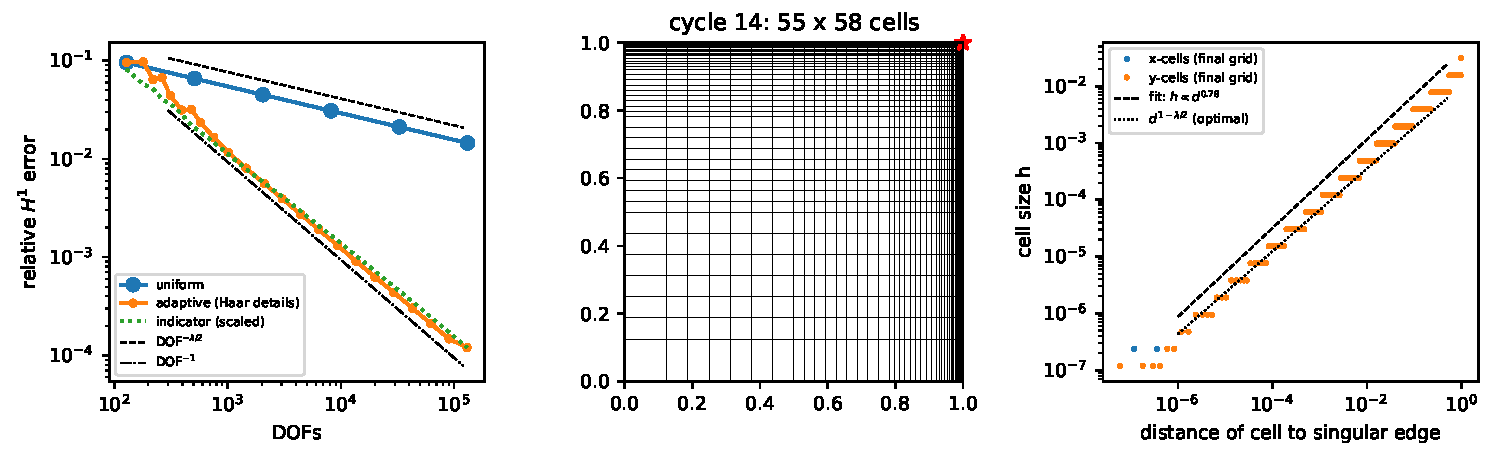
\includegraphics[width=\textwidth]{elasticity_corner.pdf}
\caption{Corner singularity, Dirichlet edges. (a) Error versus DOFs; (b) automatic grid after 14 cycles
(star: singular point); (c) cell size versus distance to the singular lines on the final grid.}\label{fig:elast}
\end{figure}

\paragraph{Traction boundaries} For the smooth solution with traction on one edge, on two adjacent
edges (including a traction--traction corner), or on two opposite edges, both the $H^1$ error and the
displacement on the traction edges converge at second order. GMRES needs 18--27 iterations,
independent of $N$ (Table~\ref{tab:tracsmooth}). With traction edges, the iteration counts grow faster
as $\nu\to\frac12$ (Table~\ref{tab:tracnu}). Since pointwise traction conditions are known to lose
accuracy for isogeometric collocation, particularly on non-uniform meshes~\cite{delorenzis2015isogeometric},
we repeated the test on graded grids (Table~\ref{tab:tracgraded}). On Chebyshev grids and on geometric
grids graded toward the traction edge ($h_{\max}/h_{\min}$ up to 85), the error remains second order,
and the displacement on the traction edges converges at second order as well. On the strongly graded
geometric grids, however, the number of GMRES iterations grows with $N$ (from 39 to 139), because the
decoupled preconditioner treats the traction rows only approximately.

\begin{table}[t]\centering\footnotesize
\caption{Traction on two adjacent edges, smooth solution, on graded grids.}\label{tab:tracgraded}
\resizebox{\textwidth}{!}{\begin{tabular}{r cccc cccc}
\toprule
 & \multicolumn{4}{c}{Chebyshev grid} & \multicolumn{4}{c}{geometric grid (toward traction edge)}\\
\cmidrule(lr){2-5}\cmidrule(lr){6-9}
$N$ & $e_{H^1}$ & rate & edge err. & its & $e_{H^1}$ & rate & $h_{\max}/h_{\min}$ & its\\
\midrule
16 & $6.73\times10^{-3}$ & -- & $8.10\times10^{-3}$ & 26 & $2.79\times10^{-2}$ & -- & 66 & 39\\
32 & $1.69\times10^{-3}$ & 1.99 & $2.04\times10^{-3}$ & 26 & $7.55\times10^{-3}$ & 1.89 & 76 & 50\\
64 & $4.23\times10^{-4}$ & 2.00 & $5.10\times10^{-4}$ & 26 & $1.93\times10^{-3}$ & 1.97 & 82 & 69\\
128 & $1.06\times10^{-4}$ & 2.00 & $1.27\times10^{-4}$ & 26 & $4.87\times10^{-4}$ & 1.99 & 85 & 139\\
\bottomrule
\end{tabular}}
\end{table}

\begin{table}[t]\centering\footnotesize
\caption{Traction boundaries, smooth solution: relative $H^1$ error for four configurations, GMRES
iterations, and the maximum displacement error on the traction edges.}\label{tab:tracsmooth}
\resizebox{\textwidth}{!}{\begin{tabular}{r cc cc cc cc }
\toprule
 & \multicolumn{2}{c}{traction on T} & \multicolumn{2}{c}{traction on T+R} & \multicolumn{2}{c}{traction on L+B} & \multicolumn{2}{c}{traction on T+B}\\
$N$ & error & rate & error & rate & error & rate & error & rate\\
\midrule
16 & $3.30\times10^{-3}$ & -- & $4.31\times10^{-3}$ & -- & $3.89\times10^{-3}$ & -- & $5.99\times10^{-3}$ & --\\
32 & $8.20\times10^{-4}$ & 2.01 & $1.08\times10^{-3}$ & 2.00 & $9.70\times10^{-4}$ & 2.00 & $1.49\times10^{-3}$ & 2.01\\
64 & $2.05\times10^{-4}$ & 2.00 & $2.70\times10^{-4}$ & 2.00 & $2.42\times10^{-4}$ & 2.00 & $3.71\times10^{-4}$ & 2.00\\
128 & $5.11\times10^{-5}$ & 2.00 & $6.75\times10^{-5}$ & 2.00 & $6.05\times10^{-5}$ & 2.00 & $9.27\times10^{-5}$ & 2.00\\
256 & $1.28\times10^{-5}$ & 2.00 & $1.69\times10^{-5}$ & 2.00 & $1.51\times10^{-5}$ & 2.00 & $2.32\times10^{-5}$ & 2.00\\
\midrule
GMRES its & \multicolumn{2}{c}{18--20} & \multicolumn{2}{c}{27--27} & \multicolumn{2}{c}{26--27} & \multicolumn{2}{c}{18--20}\\
edge error ($N{=}256$) & \multicolumn{2}{c}{$8.64\times10^{-6}$} & \multicolumn{2}{c}{$1.84\times10^{-5}$} & \multicolumn{2}{c}{$1.09\times10^{-5}$} & \multicolumn{2}{c}{$1.53\times10^{-5}$}\\
\bottomrule
\end{tabular}}
\end{table}
\begin{table}[t]\centering\footnotesize
\begin{minipage}{0.48\textwidth}\centering
\caption{1D, $u''=f$ with $u(0)$ and $u'(1)$ given: max error with an enhanced end row of weight
$\alpha$.}\label{tab:enh1d}
\resizebox{\textwidth}{!}{\begin{tabular}{r ccccc c}
\toprule
$\alpha$ & $N=32$ & $64$ & $128$ & $256$ & $512$ & rate\\
\midrule
$-1/12$ & $3.98\times10^{-4}$ & $1.02\times10^{-4}$ & $2.58\times10^{-5}$ & $6.49\times10^{-6}$ & $1.63\times10^{-6}$ & 2.00\\
0 (plain) & $1.18\times10^{-3}$ & $3.00\times10^{-4}$ & $7.58\times10^{-5}$ & $1.90\times10^{-5}$ & $4.77\times10^{-6}$ & 2.00\\
1/4 & $5.36\times10^{-3}$ & $1.36\times10^{-3}$ & $3.44\times10^{-4}$ & $8.62\times10^{-5}$ & $2.16\times10^{-5}$ & 2.00\\
1/2 & $9.54\times10^{-3}$ & $2.43\times10^{-3}$ & $6.11\times10^{-4}$ & $1.53\times10^{-4}$ & $3.84\times10^{-5}$ & 2.00\\
\bottomrule
\end{tabular}}
\end{minipage}\hfill
\begin{minipage}{0.48\textwidth}\centering
\caption{Traction on two adjacent edges: dependence on $\nu$.}\label{tab:tracnu}
\resizebox{\textwidth}{!}{\begin{tabular}{l ccc ccc}
\toprule
 & \multicolumn{3}{c}{GMRES iterations} & \multicolumn{3}{c}{$e_{H^1}$}\\
$\nu$ & $N=32$ & $64$ & $128$ & $N=32$ & $64$ & $128$\\
\midrule
0.3 & 27 & 27 & 27 & $1.08\times10^{-3}$ & $2.70\times10^{-4}$ & $6.75\times10^{-5}$\\
0.4 & 33 & 33 & 33 & $1.93\times10^{-3}$ & $4.84\times10^{-4}$ & $1.21\times10^{-4}$\\
0.45 & 44 & 44 & 44 & $3.69\times10^{-3}$ & $9.29\times10^{-4}$ & $2.33\times10^{-4}$\\
0.49 & 102 & 98 & 98 & $1.75\times10^{-2}$ & $4.49\times10^{-3}$ & $1.13\times10^{-3}$\\
0.499 & 317 & 377 & 406 & $1.37\times10^{-1}$ & $4.15\times10^{-2}$ & $1.10\times10^{-2}$\\
\bottomrule
\end{tabular}}
\end{minipage}
\end{table}

\paragraph{Singularity at the tip of a traction-free face} We now place the square so that its top edge
lies on a traction-free face of the wedge, with the singular point at the end of that face. The exact
traction on the top edge vanishes to $10^{-14}$. This is the local situation at the re-entrant corner
of the L-shaped benchmark. Uniform grids reach $1.9\times10^{-2}$ at 132k DOFs. Adaptive grids reach
$1.2\times10^{-4}$ at 149k DOFs, with a fitted rate of $\mathrm{DOF}^{-1.00}$ and 15--20 GMRES
iterations (Table~\ref{tab:tracsing}, Fig.~\ref{fig:trac}).

\begin{table}[t]\centering\footnotesize
\caption{Singularity at the tip of a traction-free face: uniform versus automatic refinement.}\label{tab:tracsing}
\begin{tabular}{rrc rrcccr}
\toprule
\multicolumn{3}{c}{uniform} & \multicolumn{6}{c}{automatic (Haar-detail indicator)}\\
\cmidrule(lr){1-3}\cmidrule(lr){4-9}
DOFs & $e_{H^1}$ & its & cycle & DOFs & $e_{H^1}$ & $h_{\min}$ & $\kappa(V)$ & its\\
\midrule
144 & $1.23\times10^{-1}$ & 18 & 0 & 144 & $1.23\times10^{-1}$ & $1.25\times10^{-1}$ & 1.0 & 18\\
544 & $8.45\times10^{-2}$ & 19 & 2 & 208 & $9.91\times10^{-2}$ & $3.12\times10^{-2}$ & 2.1 & 18\\
2112 & $5.80\times10^{-2}$ & 19 & 4 & 330 & $6.46\times10^{-2}$ & $1.56\times10^{-2}$ & 2.9 & 20\\
8320 & $3.97\times10^{-2}$ & 18 & 6 & 532 & $3.22\times10^{-2}$ & $3.91\times10^{-3}$ & 4.9 & 20\\
33024 & $2.72\times10^{-2}$ & 18 & 8 & 1040 & $1.53\times10^{-2}$ & $9.77\times10^{-4}$ & 6.7 & 20\\
131584 & $1.87\times10^{-2}$ & 17 & 10 & 2294 & $7.24\times10^{-3}$ & $2.44\times10^{-4}$ & 9.6 & 19\\
& & & 12 & 4982 & $3.42\times10^{-3}$ & $6.10\times10^{-5}$ & 13.2 & 18\\
& & & 14 & 11088 & $1.61\times10^{-3}$ & $1.53\times10^{-5}$ & 13.7 & 18\\
& & & 16 & 23320 & $7.60\times10^{-4}$ & $3.81\times10^{-6}$ & 18.4 & 17\\
& & & 18 & 48960 & $3.59\times10^{-4}$ & $9.54\times10^{-7}$ & 19.6 & 16\\
& & & 20 & 103008 & $1.70\times10^{-4}$ & $2.38\times10^{-7}$ & 26.1 & 16\\
& & & 21 & 149008 & $1.17\times10^{-4}$ & $1.19\times10^{-7}$ & 23.4 & 15\\
\bottomrule
\end{tabular}
\end{table}
\begin{figure}[t]\centering
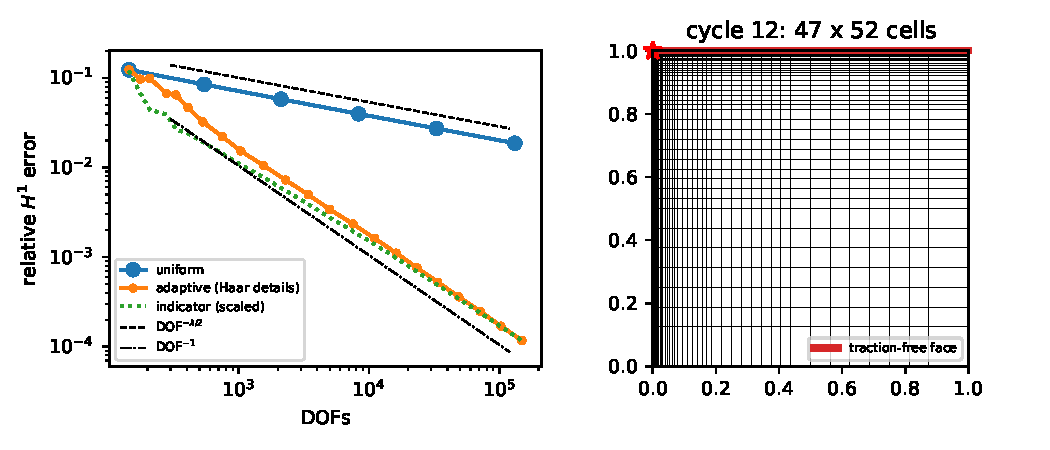
\includegraphics[width=0.8\textwidth]{elasticity_traction.pdf}
\caption{Singularity at the tip of a traction-free face (red edge; star: singular point). Left: error
versus DOFs; right: adaptive grid after 12 cycles.}\label{fig:trac}
\end{figure}

\subsection{Comparison with biquadratic finite elements}
To place the elasticity results in context, we solve the traction-free-face problem with standard
$Q_2$ (biquadratic Lagrange) Galerkin finite elements on exactly the same tensor grids: uniform, and the
sequence produced by the IHWC adaptive loop. The $Q_2$ matrices are assembled exactly as Kronecker
products of 1D matrices and solved with a sparse direct solver (SuperLU); the implementation passes the
patch test to $10^{-14}$. Fig.~\ref{fig:q2} and Table~\ref{tab:q2} show three things.
\begin{itemize}
\item On the same grid, $Q_2$ is about $1.3\times$ more accurate, but it has about $4\times$ as many
unknowns, since it has nodes at cell corners, edge midpoints and cell centres.
\item At equal numbers of unknowns, IHWC is more accurate. For example, $1.1\times10^{-3}$ with 16k
unknowns, against $2.7\times10^{-3}$ with 19k for $Q_2$.
\item At equal accuracy, the IHWC solve (GMRES with fast diagonalization) is far cheaper. An error
of about $3\times10^{-4}$ costs 0.12~s with IHWC, against 20~s for the $Q_2$ sparse direct solve.
\end{itemize}
Both methods recover the optimal adaptive rate on the IHWC-generated grids. The timing comparison
favours a structured iterative solver over a general sparse direct solver; an algebraic-multigrid
preconditioned $Q_2$ solver would narrow the gap, and wall times exclude assembly and setup in both cases.

\begin{table}[t]\centering\footnotesize
\caption{IHWC collocation versus $Q_2$ FEM on identical grids (traction-free-face singularity; every
third adaptive cycle shown). $Q_2$ was run up to $2.6\times10^5$ unknowns.}\label{tab:q2}
\begin{tabular}{r rcc rcc}
\toprule
 & \multicolumn{3}{c}{IHWC collocation (GMRES + FDM)} & \multicolumn{3}{c}{Q2 FEM (sparse direct)}\\
\cmidrule(lr){2-4}\cmidrule(lr){5-7}
cells & DOFs & $e_{H^1}$ & solve (s) & DOFs & $e_{H^1}$ & solve (s)\\
\midrule
64 & 144 & $1.23\times10^{-1}$ & 0.00 & 480 & $7.22\times10^{-2}$ & 0.00\\
130 & 280 & $6.68\times10^{-2}$ & 0.01 & 988 & $5.39\times10^{-2}$ & 0.00\\
252 & 532 & $3.22\times10^{-2}$ & 0.01 & 1944 & $2.61\times10^{-2}$ & 0.01\\
750 & 1550 & $1.05\times10^{-2}$ & 0.01 & 5880 & $8.43\times10^{-3}$ & 0.06\\
2444 & 4982 & $3.42\times10^{-3}$ & 0.02 & 19344 & $2.73\times10^{-3}$ & 0.50\\
8004 & 16182 & $1.11\times10^{-3}$ & 0.04 & 63664 & $8.80\times10^{-4}$ & 3.16\\
24327 & 48960 & $3.59\times10^{-4}$ & 0.12 & 193980 & $2.84\times10^{-4}$ & 19.77\\
74236 & 149008 & $1.17\times10^{-4}$ & 0.47 & -- & -- & --\\
\bottomrule
\end{tabular}
\end{table}
\begin{figure}[t]\centering
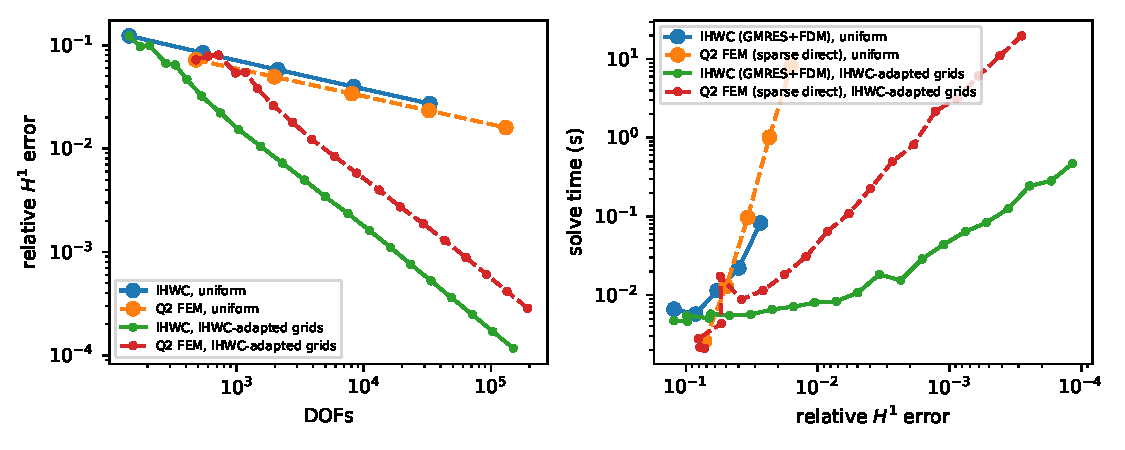
\includegraphics[width=0.85\textwidth]{ihwc_vs_q2.pdf}
\caption{IHWC collocation versus $Q_2$ FEM on identical grids. Left: error versus unknowns; right: solve
time versus error.}\label{fig:q2}
\end{figure}

\subsection{Phase-field verification}
\paragraph{Allen--Cahn shrinking circle} For $\varepsilon=0.02$ and $R_0=0.3$, the sharp-interface limit gives
$R^2(t)=R_0^2-2\varepsilon^2t$. The grid-converged slope ($128^2$ and $256^2$ agree to four digits)
deviates from this law by 0.37\%, which is consistent with the $O(\varepsilon)$ corrections to that limit.
On $64^2$, the slope differs from the converged value by 1.35\% with $D_2$ and by 0.26\% with
$D_2^{(4)}$ (Table~\ref{tab:ac}, Fig.~\ref{fig:ac}). Both the modified and the original energy decrease
at every step.

\begin{table}[t]\centering\footnotesize
\caption{Allen--Cahn shrinking circle ($\varepsilon=0.02$, $\Delta t=0.05$).}\label{tab:ac}
\resizebox{\textwidth}{!}{\begin{tabular}{l cccc}
\toprule
run & fitted $\mathrm{d}R^2/\mathrm{d}t$ & rel.\ deviation from $-2\varepsilon^2$ & $\max_n(\tilde E^{n+1}-\tilde E^n)$ & $\max_n(E_h^{n+1}-E_h^n)$\\
\midrule
$N=64$, order 2 & $-8.14\times10^{-4}$ & 1.72\% & $-8.09\times10^{-6}$ & $-1.62\times10^{-4}$\\
$N=64$, order 4 & $-8.01\times10^{-4}$ & 0.11\% & $-7.91\times10^{-6}$ & $-1.58\times10^{-4}$\\
$N=128$, order 4 & $-8.03\times10^{-4}$ & 0.36\% & $-7.92\times10^{-6}$ & $-1.58\times10^{-4}$\\
$N=256$, order 4 & $-8.03\times10^{-4}$ & 0.37\% & $-7.92\times10^{-6}$ & $-1.58\times10^{-4}$\\
\bottomrule
\end{tabular}}
\end{table}
\begin{figure}[t]\centering
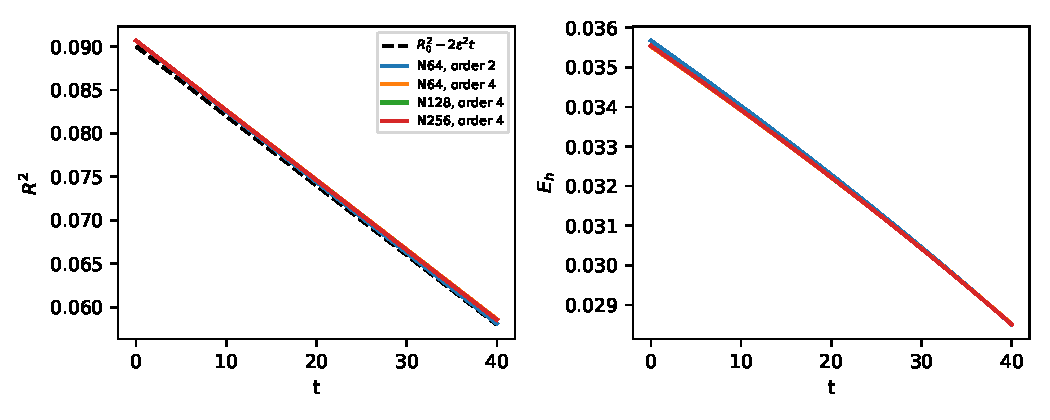
\includegraphics[width=0.72\textwidth]{allen_cahn_circle.pdf}
\caption{Allen--Cahn: $R^2(t)$ and discrete energy.}\label{fig:ac}
\end{figure}

\paragraph{Cahn--Hilliard convergence} For a smooth solution ($\varepsilon=0.05$), grids with
$N=18,54,162$ are compared with $N=486$. The ratio of 3 between grids makes the coarse midpoints a
subset of the fine ones, so no interpolation is needed. The observed orders are 2 for $D_2$ and 4 for
$D_2^{(4)}$ (Table~\ref{tab:chspace}), and the time order of SAV-BDF2 is 2 (Table~\ref{tab:chtime}).

\begin{table}[t]\centering\footnotesize
\begin{minipage}{0.52\textwidth}\centering
\caption{CH: spatial self-convergence (max norm).}\label{tab:chspace}
\begin{tabular}{r cc cc}
\toprule
 & \multicolumn{2}{c}{$D_2$} & \multicolumn{2}{c}{$D_2^{(4)}$}\\
$N$ & error & rate & error & rate\\
\midrule
18 & $7.95\times10^{-4}$ & -- & $1.36\times10^{-4}$ & --\\
54 & $9.32\times10^{-5}$ & 1.95 & $1.86\times10^{-6}$ & 3.91\\
162 & $9.40\times10^{-6}$ & 2.09 & $2.24\times10^{-8}$ & 4.02\\
\bottomrule
\end{tabular}
\end{minipage}\hfill
\begin{minipage}{0.42\textwidth}\centering
\caption{CH: temporal convergence, $N=128$.}\label{tab:chtime}
\begin{tabular}{c cc}
\toprule
$\Delta t$ & error & rate\\
\midrule
$1.60\times10^{-4}$ & $8.12\times10^{-5}$ & --\\
$8.00\times10^{-5}$ & $2.05\times10^{-5}$ & 1.99\\
$4.00\times10^{-5}$ & $5.13\times10^{-6}$ & 1.99\\
$2.00\times10^{-5}$ & $1.29\times10^{-6}$ & 2.00\\
$1.00\times10^{-5}$ & $3.21\times10^{-7}$ & 2.00\\
\bottomrule
\end{tabular}
\end{minipage}
\end{table}

\paragraph{Spinodal decomposition in 2D and 3D} With $\varepsilon=0.01$ on $256^2$ and $\varepsilon=0.02$ on
$96^3$, mass is conserved to round-off and the energy decreases monotonically
(Table~\ref{tab:spinodal}, Figs.~\ref{fig:spinodal} and~\ref{fig:ch3d}).

\begin{table}[t]\centering\footnotesize
\caption{Spinodal decomposition: conservation, energy and cost.}\label{tab:spinodal}
\begin{tabular}{l cc}
\toprule
 & 2D spinodal & 3D spinodal\\
\midrule
grid & $256^2$ & $96^3$\\
$\varepsilon$ & 0.01 & 0.02\\
steps & 5000+4500 & 1500\\
$\max_n|M_h^n-M_h^0|$ (with $M_h^0$) & $9.71\times10^{-17}$ (0.1) & $1.39\times10^{-17}$ (0.1)\\
$\max_n(\tilde E^{n+1}-\tilde E^n)$ & $-3.31\times10^{-8}$ & $-4.79\times10^{-9}$\\
$\max_n(E_h^{n+1}-E_h^n)$ (sampled) & $-8.47\times10^{-7}$ & $-2.43\times10^{-7}$\\
$\xi=r/\sqrt{E_1+C}$ range & [1.000001, 1.000349] & --\\
CPU time/step (1 core) & 2.4 ms & 67 ms\\
\bottomrule
\end{tabular}
\end{table}
\begin{figure}[t]\centering
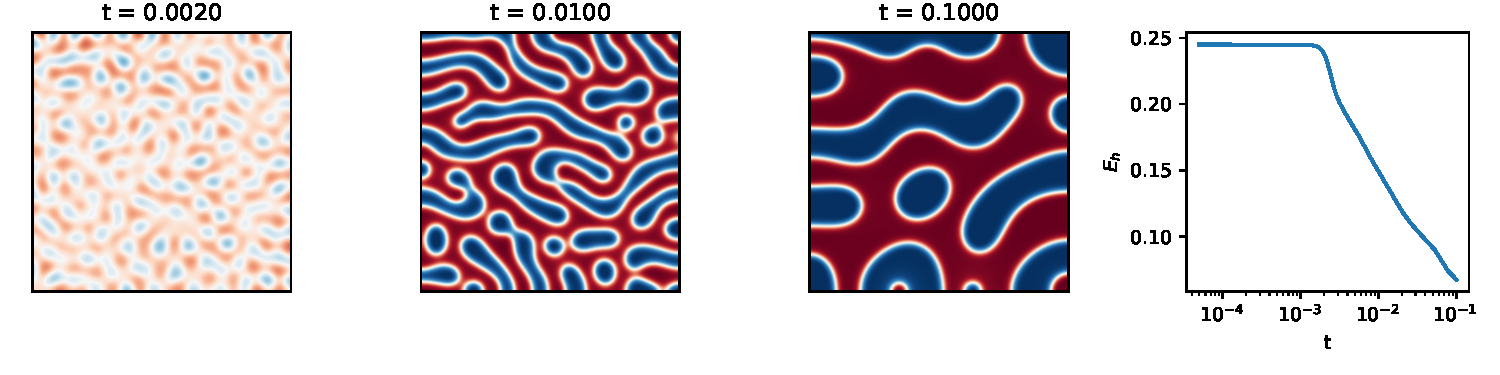
\includegraphics[width=\textwidth]{cahn_hilliard_spinodal.pdf}
\caption{CH spinodal decomposition on $256^2$: concentration at three times and discrete energy.}\label{fig:spinodal}
\end{figure}
\begin{figure}[t]\centering
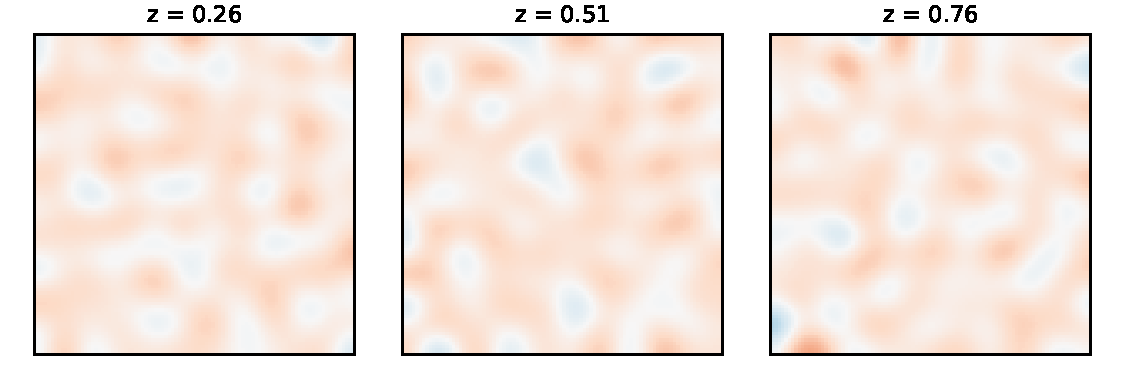
\includegraphics[width=0.62\textwidth]{cahn_hilliard_3d.pdf}
\caption{3D CH on $96^3$: slices of the concentration at the final time.}\label{fig:ch3d}
\end{figure}

\subsection{Very sharp interfaces}\label{sec:sharp}
Phase-field computations in engineering often need interfaces that are as thin as possible relative to
the domain. The relevant question is how many nodes an interface needs. Across an interface,
$u\approx\tanh(d/\sqrt2\varepsilon)$: the profile goes from $-0.76$ to $0.76$ over a distance of
$2\sqrt2\varepsilon$, and its maximum slope is $1/(\sqrt2\varepsilon)$. We therefore measure resolution in
\emph{nodes per $\sqrt2\varepsilon$}.

\paragraph{How many nodes does an interface need?} We solve the steady planar interface
$u=\tanh((x-\frac12)/\sqrt2\varepsilon)$ exactly on a discrete grid. The interface is pinned at
$x=\frac12$ by symmetry, which removes its translation mode. Fig.~\ref{fig:res} compares the 3-point finite-difference Laplacian, $D_2$, and $D_2^{(4)}$:
\begin{itemize}
\item $D_2$ is about twice as accurate as finite differences at every resolution, as
Theorem~\ref{thm:fourth} predicts.
\item $D_2^{(4)}$ pays off from about 1.5 nodes per $\sqrt2\varepsilon$. At 3.6 nodes its error is
$1.7\times10^{-4}$, compared with $4.2\times10^{-3}$ for finite differences (25$\times$ smaller). At
7.2 nodes it is $9.8\times10^{-6}$, compared with $1.1\times10^{-3}$ (110$\times$ smaller).
\item Below about 1.4 nodes per $\sqrt2\varepsilon$, the interface is under-resolved, and $D_2^{(4)}$ is not
better than $D_2$.
\end{itemize}

\begin{figure}[t]\centering
\begin{minipage}{0.45\textwidth}\centering
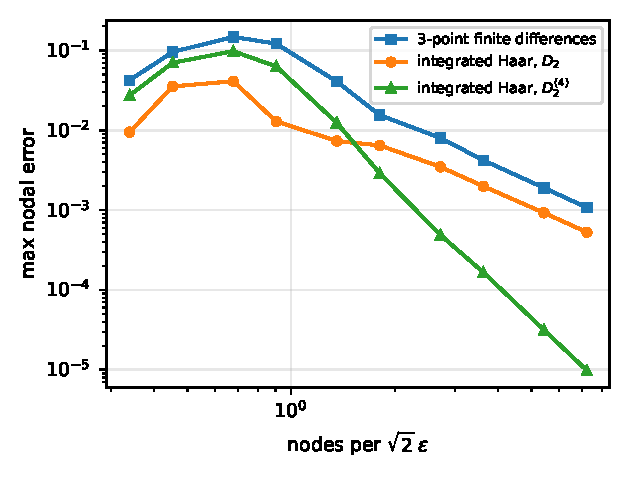
\includegraphics[width=\textwidth]{interface_resolution.pdf}
\end{minipage}\hfill
\begin{minipage}{0.52\textwidth}\centering\footnotesize
\resizebox{\textwidth}{!}{\begin{tabular}{rr ccc}
\toprule
$N$ & nodes per $\sqrt2\varepsilon$ & 3-point FD & $D_2$ & $D_2^{(4)}$\\
\midrule
48 & 0.68 & $1.47\times10^{-1}$ & $4.10\times10^{-2}$ & $9.77\times10^{-2}$\\
64 & 0.91 & $1.21\times10^{-1}$ & $1.29\times10^{-2}$ & $6.29\times10^{-2}$\\
96 & 1.36 & $4.07\times10^{-2}$ & $7.32\times10^{-3}$ & $1.24\times10^{-2}$\\
128 & 1.81 & $1.54\times10^{-2}$ & $6.45\times10^{-3}$ & $2.89\times10^{-3}$\\
192 & 2.72 & $8.02\times10^{-3}$ & $3.48\times10^{-3}$ & $4.88\times10^{-4}$\\
256 & 3.62 & $4.20\times10^{-3}$ & $1.99\times10^{-3}$ & $1.66\times10^{-4}$\\
384 & 5.43 & $1.90\times10^{-3}$ & $9.23\times10^{-4}$ & $3.16\times10^{-5}$\\
512 & 7.24 & $1.07\times10^{-3}$ & $5.28\times10^{-4}$ & $9.78\times10^{-6}$\\
\bottomrule
\end{tabular}}
\end{minipage}
\caption{Planar interface ($\varepsilon=0.01$): maximum nodal error versus nodes per $\sqrt2\varepsilon$
(left), with the data (right).}\label{fig:res}
\end{figure}

\paragraph{Allen--Cahn: a six-fold star with $\varepsilon=0.004$} The initial interface
$r=0.25+0.08\cos6\theta$ evolves under curvature flow up to $t=120$ ($\Delta t=0.1$). A $1024^2$ run with
$D_2^{(4)}$ (5.8 nodes per $\sqrt2\varepsilon$) serves as reference; coarse solutions are compared with it
at their nodes through the exact cosine-series interpolant of the reference. On $256^2$, which gives 1.45
nodes per $\sqrt2\varepsilon$, the tips with the highest curvature move visibly slower with $D_2$, while
$D_2^{(4)}$ follows the reference (Fig.~\ref{fig:star}). Table~\ref{tab:star} quantifies this:
$D_2^{(4)}$ on $256^2$ has an area error comparable to that of $D_2$ on $512^2$, with a quarter of the
unknowns. On $512^2$, $D_2^{(4)}$ is 16 times more accurate than $D_2$.

\begin{table}[t]\centering\footnotesize
\caption{Allen--Cahn star ($\varepsilon=0.004$): maximum nodal error and area error versus the $1024^2$
reference.}\label{tab:star}
\begin{tabular}{l rcc c}
\toprule
run & unknowns & max error vs.\ ref. & area error & CPU time/step\\
\midrule
$256^2$, $D_2$ & 65536 & $1.36\times10^{-1}$ & $2.43\times10^{-4}$ & 2.4 ms\\
$256^2$, $D_2^{(4)}$ & 65536 & $5.27\times10^{-2}$ & $6.07\times10^{-5}$ & 2.4 ms\\
$512^2$, $D_2$ & 262144 & $4.12\times10^{-2}$ & $6.88\times10^{-5}$ & 15.1 ms\\
$512^2$, $D_2^{(4)}$ & 262144 & $2.63\times10^{-3}$ & $4.23\times10^{-6}$ & 14.0 ms\\
$1024^2$, $D_2^{(4)}$ (ref.) & 1048576 & -- & -- & 73 ms\\
\bottomrule
\end{tabular}
\end{table}
\begin{figure}[t]\centering
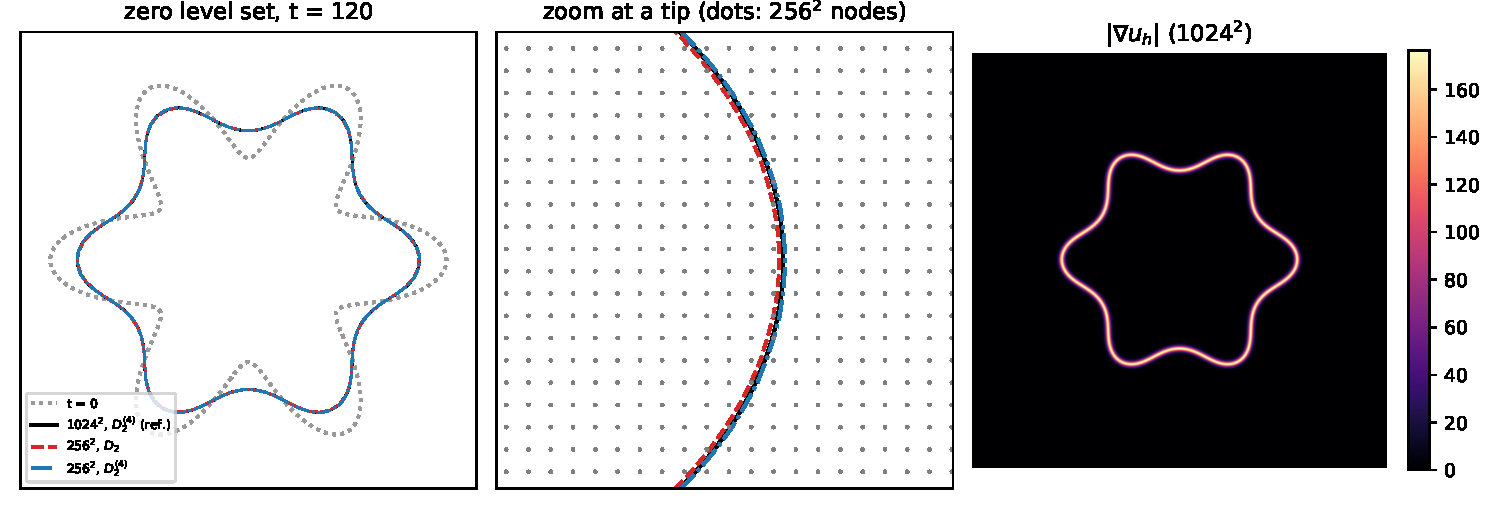
\includegraphics[width=\textwidth]{allen_cahn_star.pdf}
\caption{Allen--Cahn star, $\varepsilon=0.004$. Left: zero level sets at $t=0$ and $t=120$; middle: zoom at
a tip with the $256^2$ nodes; right: gradient magnitude of the reference solution.}\label{fig:star}
\end{figure}

\paragraph{Cahn--Hilliard with $\varepsilon=0.0015$ on $1024^2$} This gives only 2.2 nodes per
$\sqrt2\varepsilon$: the whole interface, from $u=-0.76$ to $0.76$, spans about four nodes. Starting from a
random mixture, we use stabilized SAV ($S=4$) with three stages of 1500 steps each, at
$\Delta t=2\times10^{-7}$, $2\times10^{-6}$ and $2\times10^{-5}$, up to $t=0.033$.
Fig.~\ref{fig:chsharp} and Table~\ref{tab:chsharp} show that:
\begin{itemize}
\item mass is conserved to $10^{-17}$;
\item both the modified and the original energy decrease at every step;
\item $|u_h|$ stays below 1.03, so there are no visible overshoots;
\item the nodal profile across an interface coincides with the $\tanh$ profile;
\item the maximum computed gradient (467) matches the exact planar-interface value $1/(\sqrt2\varepsilon)=471$.
\end{itemize}
Table~\ref{tab:savstab} shows what happens without stabilization, when the computation is restarted at
$t=0.0033$.

\begin{table}[t]\centering\footnotesize
\begin{minipage}{0.48\textwidth}\centering
\caption{CH with $\varepsilon=0.0015$ on $1024^2$, stabilized SAV ($S=4$).}\label{tab:chsharp}
\resizebox{\textwidth}{!}{\begin{tabular}{l c}
\toprule
grid / $\varepsilon$ & $1024^2$ / 0.0015\\
nodes per $\sqrt2\varepsilon$ & 2.17\\
time steps & 1500$\times$$2.00\times10^{-7}$ + 1500$\times$$2.00\times10^{-6}$ + 1500$\times$$2.00\times10^{-5}$\\
$\max_n|M_h^n-M_h^0|$ & $6.49\times10^{-18}$\\
$\max_n(\tilde E^{n+1}-\tilde E^n)$ & $-7.20\times10^{-8}$\\
$\max|\nabla u_h|$ / planar-interface value $1/(\sqrt2\varepsilon)$ & 467 / 471\\
CPU time per step (1 core) & 101 ms\\
\bottomrule
\end{tabular}}
\end{minipage}\hfill
\begin{minipage}{0.48\textwidth}\centering
\caption{Plain ($S=0$) versus stabilized ($S=4$) SAV, 150 steps from $t=0.0033$.}\label{tab:savstab}
\resizebox{\textwidth}{!}{\begin{tabular}{cc cccc}
\toprule
$S$ & $\Delta t$ & $\max|u_h|$ & $E_h$: start $\to$ end & $\xi=r/\sqrt{E_1+C}$ & $\max_n(\tilde E^{n+1}-\tilde E^n)$\\
\midrule
0 & $2.00\times10^{-5}$ & 77.33 & 0.0617 $\to$ 503.6812 & -0.00003 & $-4.59\times10^{-5}$\\
0 & $5.00\times10^{-6}$ & 122.58 & 0.0617 $\to$ 801.4332 & -0.00002 & $-3.23\times10^{-5}$\\
4 & $2.00\times10^{-5}$ & 1.04 & 0.0617 $\to$ 0.0503 & 1.00002 & $-5.02\times10^{-5}$\\
4 & $5.00\times10^{-6}$ & 1.04 & 0.0617 $\to$ 0.0578 & 1.00000 & $-2.27\times10^{-5}$\\
\bottomrule
\end{tabular}}
\end{minipage}
\end{table}
\begin{figure}[t]\centering
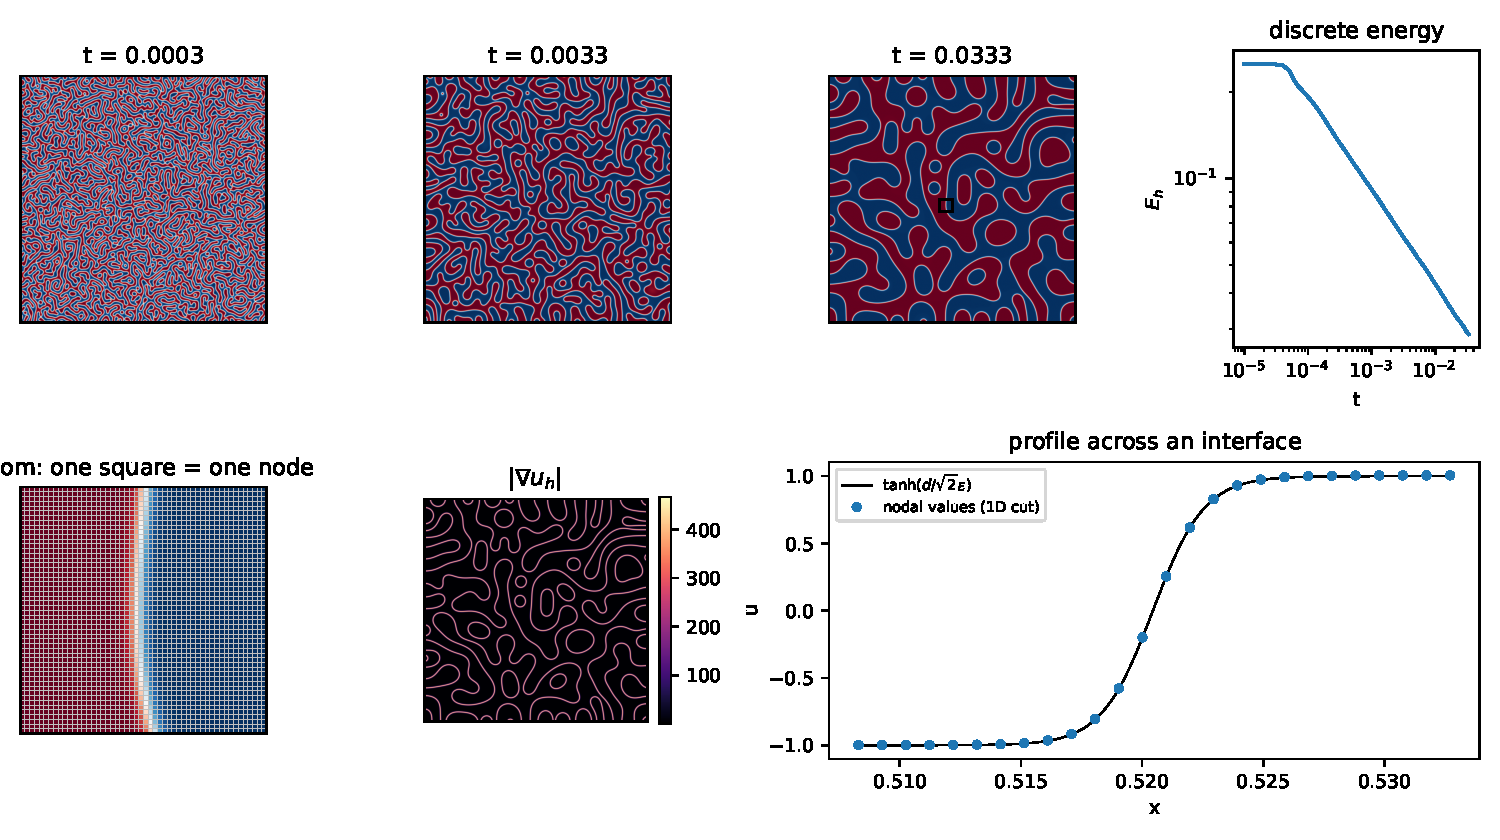
\includegraphics[width=\textwidth]{cahn_hilliard_sharp.pdf}
\caption{CH with $\varepsilon=0.0015$ on $1024^2$. Top: concentration at three times (the box marks the
zoomed region) and discrete energy. Bottom: zoom in which each square is one node; gradient magnitude;
nodal values along a grid line crossing an interface, compared with the $\tanh$ profile.}\label{fig:chsharp}
\end{figure}

\subsection{Comparison with other discretizations on uniform grids}\label{sec:compare}
All the uniform-grid operators considered here are diagonalized by the same cosine transform. The
3-point difference, IHWC $D_2$ and $D_2^{(4)}$, the compact Pad\'e operator, and the cosine
pseudo-spectral operator therefore differ only in the eigenvalues used in Algorithm~2. This makes an
exactly fair comparison possible: same SAV scheme, same time step, same cost per step.
Table~\ref{tab:compare} and Fig.~\ref{fig:compare} lead to the following conclusions.
\begin{itemize}
\item IHWC $D_2$ is consistently about $2\times$ more accurate than the 3-point difference, at the same
cost.
\item The Pad\'e operator is about $1.4\times$ more accurate than $D_2^{(4)}$, as predicted by the error
constants.
\item For problems on uniform boxes with zero-flux or periodic conditions, the pseudo-spectral operator
is far more accurate. It reaches round-off on the smooth Cahn--Hilliard case with $N=54$, and it is
$15\times$ more accurate than $D_2^{(4)}$ on the $512^2$ star. Its overshoot is negligible
($|u|\le1.00003$).
\end{itemize}
We therefore do not advocate IHWC for phase-field problems on uniform boxes with zero-flux or periodic
conditions, where pseudo-spectral methods are the natural choice. The value of the formulation lies
elsewhere. It is a single, structure-preserving discretization that also covers graded and adaptively
refined grids, prescribed values and traction conditions, and singular solutions, where spectral
methods do not apply directly. It also gives the many existing HWCM codes a direct route to fast and
provably stable solvers.

\begin{table}[t]\centering\footnotesize
\caption{Uniform-grid discretizations within the identical SAV-BDF2 solver. Left: smooth CH (reference:
pseudo-spectral, $N=486$); right: AC star (reference: IHWC $D_2^{(4)}$, $1024^2$).}\label{tab:compare}
\resizebox{\textwidth}{!}{\begin{tabular}{l ccc cccc}
\toprule
 & \multicolumn{3}{c}{CH smooth, max error} & \multicolumn{4}{c}{AC star, $\varepsilon=0.004$}\\
\cmidrule(lr){2-4}\cmidrule(lr){5-8}
scheme & $N=18$ & $54$ & $162$ & error $256^2$ & error $512^2$ & area $256^2$ & area $512^2$\\
\midrule
3-point FD & $1.63\times10^{-3}$ & $1.89\times10^{-4}$ & $2.12\times10^{-5}$ & $3.89\times10^{-1}$ & $8.85\times10^{-2}$ & $6.02\times10^{-4}$ & $1.46\times10^{-4}$\\
IHWC $D_2$ & $7.96\times10^{-4}$ & $9.44\times10^{-5}$ & $1.06\times10^{-5}$ & $1.36\times10^{-1}$ & $4.12\times10^{-2}$ & $2.43\times10^{-4}$ & $6.88\times10^{-5}$\\
IHWC $D_2^{(4)}$ & $1.36\times10^{-4}$ & $1.86\times10^{-6}$ & $2.27\times10^{-8}$ & $5.27\times10^{-2}$ & $2.63\times10^{-3}$ & $6.07\times10^{-5}$ & $4.23\times10^{-6}$\\
compact 4th order (Pad\'e) & $9.42\times10^{-5}$ & $1.31\times10^{-6}$ & $1.60\times10^{-8}$ & $3.65\times10^{-2}$ & $1.78\times10^{-3}$ & $3.77\times10^{-5}$ & $2.88\times10^{-6}$\\
cosine pseudo-spectral & $4.40\times10^{-7}$ & $3.39\times10^{-15}$ & $1.61\times10^{-15}$ & $1.52\times10^{-2}$ & $1.68\times10^{-4}$ & $1.24\times10^{-5}$ & $2.72\times10^{-7}$\\
\bottomrule
\end{tabular}}
\end{table}
\begin{figure}[t]\centering
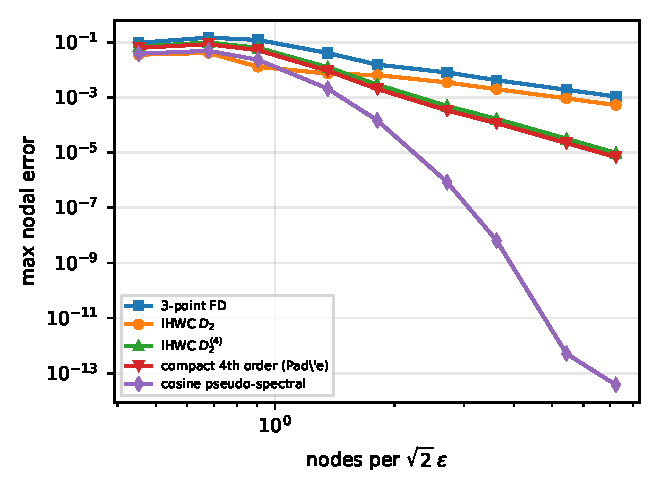
\includegraphics[width=0.5\textwidth]{scheme_comparison.pdf}
\caption{Planar interface: maximum nodal error versus resolution for five discretizations.}\label{fig:compare}
\end{figure}

\subsection{Performance}
Table~\ref{tab:perf} reports the time per CH step. On one CPU core, the cosine-transform variant
processes $1$--$3\times10^7$ unknowns per second. \todo{GPU columns pending: run \texttt{python experiments/run\_all.py --only E6 --gpu} and \texttt{python experiments/make\_tables.py} on a CUDA machine.}

\begin{table}[t]\centering\footnotesize
\caption{Time per Cahn--Hilliard SAV-BDF2 step ($D_2^{(4)}$).}\label{tab:perf}
\begin{tabular}{rr r cc cc cc}
\toprule
 & & & \multicolumn{2}{c}{CPU, 1 core, fp64} & \multicolumn{2}{c}{GPU, fp64} & \multicolumn{2}{c}{GPU, fp32}\\
$d$ & $N$ & unknowns & GEMM & DCT & GEMM & DCT & GEMM & DCT\\
\midrule
2 & 128 & 16384 & 0.74 & 0.53 & \textit{pending} & \textit{pending} & \textit{pending} & \textit{pending}\\
2 & 256 & 65536 & 4.14 & 2.02 & \textit{pending} & \textit{pending} & \textit{pending} & \textit{pending}\\
2 & 512 & 262144 & 28.80 & 12.64 & \textit{pending} & \textit{pending} & \textit{pending} & \textit{pending}\\
2 & 1024 & 1048576 & 182.56 & 55.51 & \textit{pending} & \textit{pending} & \textit{pending} & \textit{pending}\\
2 & 2048 & 4194304 & -- & 370.38 & \textit{pending} & \textit{pending} & \textit{pending} & \textit{pending}\\
3 & 32 & 32768 & 1.16 & 1.44 & \textit{pending} & \textit{pending} & \textit{pending} & \textit{pending}\\
3 & 64 & 262144 & 16.89 & 14.75 & \textit{pending} & \textit{pending} & \textit{pending} & \textit{pending}\\
3 & 128 & 2097152 & 176.91 & 160.08 & \textit{pending} & \textit{pending} & \textit{pending} & \textit{pending}\\
\bottomrule
\end{tabular}
\end{table}

%==========================================================================
\section{Practical guidelines}\label{sec:guide}
%==========================================================================
Table~\ref{tab:guide} summarizes the choices that worked in our computations.

\begin{table}[H]\centering\footnotesize
\caption{Practical recommendations.}\label{tab:guide}
\begin{tabular}{p{0.3\textwidth}p{0.64\textwidth}}
\toprule
Decision & Recommendation\\
\midrule
Plain or corrected operator & Use $D_2^{(4)}$ for zero-flux or periodic problems: it costs nothing extra. With general prescribed values, use $D_2$ (the correction does not raise the order there).\\
When \emph{not} to use IHWC & Smooth or phase-field problems on uniform boxes with zero-flux or periodic conditions: a cosine pseudo-spectral operator is far more accurate at the same cost (Section~\ref{sec:compare}).\\
Interface resolution & At least 1.5 nodes per $\sqrt2\varepsilon$ with $D_2^{(4)}$. Expect a nodal error of about $10^{-3}$ at 2--3 nodes, and about $10^{-4}$ at 3.5 nodes (Fig.~\ref{fig:res}).\\
Time stepping (AC/CH) & SAV-BDF2 with stabilization $S\approx4$. Monitor $\xi=r/\sqrt{E_{1,h}+C}$: if it leaves $[0.999,1.001]$, reduce $\Delta t$. Start with small steps from random initial data and increase $\Delta t$ as the structure coarsens (restart BDF1 at each change).\\
Solver & Uniform grids: cosine/sine transforms. Graded grids: fast diagonalization (GEMM) with a check that the spectrum is real and $\kappa(V)$ small. Coupled systems (elasticity): GMRES with the block preconditioner.\\
Adaptivity (singularities) & Haar-detail indicator, D\"orfler $\theta\approx0.6$, neighbour ratio $\le2$, starting from $8\times8$ cells.\\
Traction conditions & Plain collocation at edge midpoints, with no enhancement; normal-stress conditions at traction--traction corners.\\
Near incompressibility & Avoid $\nu>0.45$ with the present formulation (Tables~\ref{tab:nu} and~\ref{tab:tracnu}).\\
\bottomrule
\end{tabular}
\end{table}

%==========================================================================
\section{Limitations and outlook}\label{sec:limits}
%==========================================================================
\begin{itemize}
\item \emph{Geometry.} The fast solvers require rectangular domains. Non-convex domains such as the full
L-shaped domain, and curved boundaries, need multi-patch coupling or geometry maps. The local corner
structure of the L-shape is covered by the traction-free-face test.
\item \emph{Locality of refinement.} Tensor refinement extends refinement lines across the domain. For
point singularities this costs only a constant factor, and the optimal rate is retained. For interfaces
that move through the domain, local refinement would be preferable, but integrated Haar functions are
not compactly supported, so it would require a different basis (for example, truncated hierarchical
B-splines).
\item \emph{Scope of the comparisons.} We compared with $Q_2$ FEM on identical grids and with
finite-difference, compact and pseudo-spectral operators on uniform grids
(Sections~\ref{sec:compare} and the $Q_2$ comparison). A comparison with adaptive hierarchical IGA
collocation~\cite{schillinger2013isogeometric} and with AMG-preconditioned FEM is still missing.
\item \emph{Theory on graded grids.} There, $D_2$ is not symmetric. Real spectra were observed in every
computation, but this is not proved, and the energy analysis is restricted to uniform grids.
\item \emph{Near incompressibility} requires a mixed displacement--pressure formulation, or a
preconditioner that couples $u$ and $v$.
\end{itemize}

%==========================================================================
\section{Conclusions}
%==========================================================================
An exact three-term identity shows that Haar wavelet collocation is quadratic-spline collocation. It
replaces the dense HWCM matrices by tridiagonal ones and gives access to fast tensor solvers, a free
fourth-order correction, exact mass conservation, and provable energy stability. With stabilized SAV
time stepping, Allen--Cahn and Cahn--Hilliard interfaces are resolved accurately down to about two
nodes per $\sqrt2\varepsilon$, at a cost of two fast transforms per step. For elastostatics with Dirichlet
and traction edges, preconditioned GMRES converges in a mesh-independent number of iterations, and
automatic refinement from Haar detail coefficients recovers optimal convergence at corner singularities.

\section*{Code and data availability}
Code, tests and the scripts that produce every table and figure are available at \todo{repository URL /
Zenodo DOI}. Dependencies are listed in \texttt{requirements.txt} (CPU) and
\texttt{requirements-gpu.txt} (GPU, CuPy).

\section*{Declaration of competing interest}
The author declares no known competing financial interests or personal relationships that could have
appeared to influence the work reported in this paper.

\clearpage
%==========================================================================
\appendix
\section{Proofs for Section~\ref{sec:method}}\label{app:ops}
%==========================================================================
\subsection{Theorem~\ref{thm:identity} and Corollary~\ref{cor:ops}}\label{app:identity}
\begin{proof}[Proof of Theorem~\ref{thm:identity}]
Let $\sigma_k=s'(t_k)$. On $I_k$, $s'(x)=\sigma_k+c_k(x-t_k)=\sigma_{k-1}+c_k(x-t_{k-1})$, hence
$\sigma_k-\sigma_{k-1}=c_kh_k$. Integrating $s'$ from $m_k$ to $m_{k+1}$ across $t_k$,
\[
U_{k+1}-U_k=\int_{m_k}^{t_k}\!\big(\sigma_k+c_k(x-t_k)\big)dx+\int_{t_k}^{m_{k+1}}\!\big(\sigma_k+c_{k+1}(x-t_k)\big)dx
=\sigma_kd_k-\frac{c_kh_k^2}{8}+\frac{c_{k+1}h_{k+1}^2}{8}.
\]
Dividing by $d_k$, subtracting the same relation for $k-1$, and using
$\sigma_k-\sigma_{k-1}=c_kh_k$ gives~\eqref{eq:interior}. At the left end,
$U_1-g_0=\sigma_0h_1/2+c_1h_1^2/8$, so $2(U_1-g_0)/h_1=\sigma_0+c_1h_1/4$; subtracting this from the
relation for $(U_2-U_1)/d_1$ gives~\eqref{eq:dirrow}. If $\sigma_0=0$, then $\sigma_1=c_1h_1$
and~\eqref{eq:neurow} follows. The right end is analogous. The expressions for $s'(m_k)$ and for the
end slopes follow from $s'=\sigma_0+\int s''$.
\end{proof}
\begin{proof}[Proof of Corollary~\ref{cor:ops}]
The off-diagonal entries of column $k$ sum to $h_k^2/(8d_{k-1})+h_k^2/(8d_k)$, so the column-dominance
margin is $h_k-h_k^2/(4d_{k-1})-h_k^2/(4d_k)>0$, because $d_j>h_k/2$. For an end column with a
prescribed value, the margin is $3h_1/4-h_1^2/(4d_1)>h_1/4$; for a zero-slope end column it is
$h_1-h_1^2/(4d_1)>h_1/2$. With values prescribed at both ends, $L$ is a symmetric negative definite
three-point matrix, so $LU=Af-b_0g_0-b_1g_1$ has a unique solution.
\end{proof}

\subsection{Proposition~\ref{prop:uniform}}\label{app:uniform}
\begin{proof}
With $h_k=h$ we have $d_k=h$, and the coefficients of~\eqref{eq:interior}--\eqref{eq:neurow} become
$h(\frac18,\frac68,\frac18)$, $h(\frac58,\frac18)$ and $h(\frac78,\frac18)$. These are the rows of
$h(I+\delta^2/8)$, while the left-hand sides are the rows of $\delta^2/h$. Since $I+\delta^2/8$ is a
polynomial in the symmetric matrix $\delta^2$, the two commute, and
$D_2=h^{-2}(I+\delta^2/8)^{-1}\delta^2$ is symmetric. The end rows of $\delta^2$ correspond to ghost values
$U_0=-U_1$ (odd reflection) or $U_0=U_1$ (even reflection), whose eigenvectors are the DST-II and DCT-II
vectors with eigenvalues $\mu_k\in[-4,0]$. Finally, $\mu\mapsto8\mu/(8+\mu)$ maps $[-4,0]$ monotonically
onto $[-8,0]$.
\end{proof}

\subsection{Theorem~\ref{thm:fourth}}\label{app:fourth}
\begin{proof}
By the reflection property, the zero-slope matrices act on $U$ as the circulant matrices of the
$2N$-point periodic grid act on the even extension. For a sampled exponential $e^{i\omega x}$, the
circulant $D_2$ has eigenvalue $\lambda(\omega h)/h^2$, with $2\pi$-periodic analytic symbol
$\lambda(\theta)=8\mu/(8+\mu)$, $\mu=-4\sin^2(\theta/2)=-\theta^2+\theta^4/12+O(\theta^6)$. Hence
$\lambda=\mu-\mu^2/8+O(\mu^3)=-\theta^2-\theta^4/24+O(\theta^6)$, which gives the first statement mode by
mode. The symbol of $D_2^{(4)}$ is $\lambda+\lambda^2/24=-\theta^2+O(\theta^6)$, so
$|\lambda_4(\omega h)/h^2+\omega^2|\le Ch^4\omega^6$ for $|\omega h|\le\pi$. For $|\omega h|>\pi$ this
holds trivially, because $|\lambda_4|\le16/3$. Summing over the rapidly decaying Fourier coefficients of
the smooth periodic extension gives the $O(h^4)$ bound. The spectral statement follows because
$\lambda+h^2\lambda^2/24\le0$ for $\lambda\in[-24/h^2,0]$. Prescribed values with odd extensions are
treated identically.
\end{proof}

\subsection{Proposition~\ref{prop:mass}}\label{app:mass}
\begin{proof}
From~\eqref{eq:interior} and~\eqref{eq:neurow}, column $k$ of $A$ sums to
$h_k-\frac{h_k^2}{8d_{k-1}}-\frac{h_k^2}{8d_k}+\frac{h_k^2}{8d_{k-1}}+\frac{h_k^2}{8d_k}=h_k$, i.e.\
$\mathbf 1^{\mathsf T}A=h^{\mathsf T}$. Hence $h^{\mathsf T}D_2=\mathbf 1^{\mathsf T}L=0$, because the columns
of the zero-slope difference matrix sum to zero. On uniform grids,
$\int_{I_k}s=hU_k+h^3c_k/24$ exactly, and $\sum_kh\,c_k=s'(b)-s'(a)=0$.
\end{proof}

%==========================================================================
\section{Proof of Theorem~\ref{thm:energy}}\label{app:energy}
%==========================================================================
\begin{proof}
\emph{Solvability.} Eliminating $\mu$ gives
$Mu^{n+1}=g+2\Delta t\,S\,G_h\bar u-2\Delta t\,r^{n+1}G_h\bar b$ with
$M=3I+2\Delta t\,G_h(\varepsilon^2K+SI)$. The matrix $M$ is symmetric positive definite, because $G_h$ and $K$ commute and are positive semidefinite.
Writing $u^{n+1}=p+r^{n+1}q$ and substituting into~\eqref{eq:sav2} gives a scalar equation for
$r^{n+1}$ whose coefficient is $3-\tfrac32\langle\bar b,q\rangle_h\ge3$, since
$\langle\bar b,q\rangle_h=-2\Delta t\langle\bar b,M^{-1}G_h\bar b\rangle_h\le0$.

\emph{Mass.} For CH, $\langle K\mu,1\rangle_h=\langle\mu,K1\rangle_h=0$, so
$\langle3u^{n+1}-4u^n+u^{n-1},1\rangle_h=0$. Since the BDF1 first step conserves mass, induction
gives conservation, and Proposition~\ref{prop:mass} identifies the discrete sum with the integral.

\emph{Energy.} Take the inner product of~\eqref{eq:sav1} with $2\Delta t\,\mu^{n+1}$. The left-hand side
is $-2\Delta t\langle G_h\mu,\mu\rangle_h\le0$. On the right-hand side, write $a=u^{n+1}$, $b=u^n$,
$c=u^{n-1}$, and use three identities:
\begin{align*}
2\langle3a-4b+c,Ka\rangle_h&=\|a\|_K^2-\|b\|_K^2+\|2a-b\|_K^2-\|2b-c\|_K^2+\|a-2b+c\|_K^2,\\
\langle3a-4b+c,a-2b+c\rangle_h&=\|a-b\|_h^2-\|b-c\|_h^2+2\|a-2b+c\|_h^2,
\end{align*}
where the second follows from $(3x-y)(x-y)=x^2-y^2+2(x-y)^2$ with $x=a-b$ and $y=b-c$. The third is
the scalar version of the first, applied to~\eqref{eq:sav2} multiplied by $2r^{n+1}$. Collecting
terms gives
\[
\tilde E^{n+1}-\tilde E^n=-\Delta t\langle G_h\mu^{n+1},\mu^{n+1}\rangle_h-\tfrac{\varepsilon^2}{4}\|a-2b+c\|_K^2
-\tfrac12(r^{n+1}-2r^n+r^{n-1})^2-S\|a-2b+c\|_h^2\le0.
\]
The same argument applies to BDF1 and to both $D_2$ and $D_2^{(4)}$, since only the symmetry and
semidefiniteness of $K$ in $\langle\cdot,\cdot\rangle_h$ (Proposition~\ref{prop:uniform},
Theorem~\ref{thm:fourth}) are used.
\end{proof}

%==========================================================================
\begin{thebibliography}{99}
\bibitem{chen1997haar} C.F. Chen, C.H. Hsiao, Haar wavelet method for solving lumped and distributed-parameter systems, IEE Proc. Control Theory Appl. 144 (1997) 87--94.
\bibitem{lepik2005numerical} \"U. Lepik, Numerical solution of differential equations using Haar wavelets, Math. Comput. Simul. 68 (2005) 127--143.
\bibitem{lepik2007application} \"U. Lepik, Application of the Haar wavelet transform to solving integral and differential equations, Proc. Estonian Acad. Sci. Phys. Math. 56 (2007) 28--46.
\bibitem{lepik2011solving} \"U. Lepik, Solving PDEs with the aid of two-dimensional Haar wavelets, Comput. Math. Appl. 61 (2011) 1873--1879.
\bibitem{lepik2014book} \"U. Lepik, H. Hein, Haar Wavelets: With Applications, Springer, Cham, 2014.
\bibitem{majak2015accuracy} J. Majak, B. Shvartsman, K. Karjust, M. Mikola, A. Haavaj\~oe, M. Pohlak, On the accuracy of the Haar wavelet discretization method, Compos. B Eng. 80 (2015) 321--327.
\bibitem{majak2015convergence} J. Majak, B.S. Shvartsman, M. Kirs, M. Pohlak, H. Herranen, Convergence theorem for the Haar wavelet based discretization method, Compos. Struct. 126 (2015) 227--232.
\bibitem{majak2018higher} J. Majak, M. Pohlak, K. Karjust, M. Eerme, J. Kurnitski, B.S. Shvartsman, New higher order Haar wavelet method: Application to FGM structures, Compos. Struct. 201 (2018) 72--78.
\bibitem{ratas2021solving} M. Ratas, J. Majak, A. Salupere, Solving nonlinear boundary value problems using the higher order Haar wavelet method, Mathematics 9 (2021) 2809.
\bibitem{dubeau2004nonuniform} F. Dubeau, S. Elmejdani, R. Ksantini, Non-uniform Haar wavelets, Appl. Math. Comput. 159 (2004) 675--693.
\bibitem{lepik2008nonuniform} \"U. Lepik, Solving integral and differential equations by the aid of non-uniform Haar wavelets, Appl. Math. Comput. 198 (2008) 326--332.
\bibitem{oruc2019nonuniform} \"O. Oru\c{c}, A non-uniform Haar wavelet method for numerically solving two-dimensional convection-dominated equations and two-dimensional near singular elliptic equations, Comput. Math. Appl. 77 (2019) 1799--1820.
\bibitem{houstis1988quadratic} E.N. Houstis, C.C. Christara, J.R. Rice, Quadratic-spline collocation methods for two-point boundary value problems, Int. J. Numer. Methods Eng. 26 (1988) 935--952.
\bibitem{christara1994quadratic} C.C. Christara, Quadratic spline collocation methods for elliptic partial differential equations, BIT 34 (1994) 33--61.
\bibitem{christara2006optimal} C.C. Christara, K.S. Ng, Optimal quadratic and cubic spline collocation on nonuniform partitions, Computing 76 (2006) 227--257.
\bibitem{christara2006adaptive} C.C. Christara, K.S. Ng, Adaptive techniques for spline collocation, Computing 76 (2006) 259--277.
\bibitem{christara2002fast} C.C. Christara, K.S. Ng, Fast Fourier transform solvers and preconditioners for quadratic spline collocation, BIT 42 (2002) 702--739.
\bibitem{auricchio2010isogeometric} F. Auricchio, L. Beir\~ao da Veiga, T.J.R. Hughes, A. Reali, G. Sangalli, Isogeometric collocation methods, Math. Models Methods Appl. Sci. 20 (2010) 2075--2107.
\bibitem{schillinger2013isogeometric} D. Schillinger, J.A. Evans, A. Reali, M.A. Scott, T.J.R. Hughes, Isogeometric collocation: Cost comparison with Galerkin methods and extension to adaptive hierarchical NURBS discretizations, Comput. Methods Appl. Mech. Engrg. 267 (2013) 170--232.
\bibitem{anitescu2015isogeometric} C. Anitescu, Y. Jia, Y.J. Zhang, T. Rabczuk, An isogeometric collocation method using superconvergent points, Comput. Methods Appl. Mech. Engrg. 284 (2015) 1073--1097.
\bibitem{gomez2016variational} H. Gomez, L. De Lorenzis, The variational collocation method, Comput. Methods Appl. Mech. Engrg. 309 (2016) 152--181.
\bibitem{delorenzis2015isogeometric} L. De Lorenzis, J.A. Evans, T.J.R. Hughes, A. Reali, Isogeometric collocation: Neumann boundary conditions and contact, Comput. Methods Appl. Mech. Engrg. 284 (2015) 21--54.
\bibitem{lynch1964direct} R.E. Lynch, J.R. Rice, D.H. Thomas, Direct solution of partial difference equations by tensor product methods, Numer. Math. 6 (1964) 185--199.
\bibitem{bartels1972solution} R.H. Bartels, G.W. Stewart, Solution of the matrix equation $AX+XB=C$, Commun. ACM 15 (1972) 820--826.
\bibitem{sangalli2016isogeometric} G. Sangalli, M. Tani, Isogeometric preconditioners based on fast solvers for the Sylvester equation, SIAM J. Sci. Comput. 38 (2016) A3644--A3671.
\bibitem{shen2018scalar} J. Shen, J. Xu, J. Yang, The scalar auxiliary variable (SAV) approach for gradient flows, J. Comput. Phys. 353 (2018) 407--416.
\bibitem{dorfler1996convergent} W. D\"orfler, A convergent adaptive algorithm for Poisson's equation, SIAM J. Numer. Anal. 33 (1996) 1106--1124.
\bibitem{williams1952stress} M.L. Williams, Stress singularities resulting from various boundary conditions in angular corners of plates in extension, J. Appl. Mech. 19 (1952) 526--528.
\bibitem{grisvard1985elliptic} P. Grisvard, Elliptic Problems in Nonsmooth Domains, Pitman, Boston, 1985.
\bibitem{babuska1979direct} I. Babu\v{s}ka, R.B. Kellogg, J. Pitk\"aranta, Direct and inverse error estimates for finite elements with mesh refinements, Numer. Math. 33 (1979) 447--471.
\bibitem{apel1999anisotropic} T. Apel, Anisotropic Finite Elements: Local Estimates and Applications, Teubner, Stuttgart, 1999.
\end{thebibliography}
\end{document}
